\documentclass{article}

% if you need to pass options to natbib, use, e.g.:
%     \PassOptionsToPackage{numbers, compress}{natbib}
% before loading neurips_2026

% The authors should use one of these tracks.
% Before accepting by the NeurIPS conference, select one of the options below.
% 0. "default" for submission
% \usepackage{neurips_2026}
% the "default" option is equal to the "main" option, which is used for the Main Track with double-blind reviewing.
% 1. "main" option is used for the Main Track
%  \usepackage[main]{neurips_2026}
% 2. "position" option is used for the Position Paper Track
%  \usepackage[position]{neurips_2026}
% 3. "eandd" option is used for the Evaluations & Datasets Track
 % \usepackage[eandd]{neurips_2026}
 % if you need to opt-in for a single-blind submission in the E&D track:
 %\usepackage[eandd, nonanonymous]{neurips_2026}
% 4. "creativeai" option is used for the Creative AI Track
%  \usepackage[creativeai]{neurips_2026}
% 5. "sglblindworkshop" option is used for the Workshop with single-blind reviewing
 % \usepackage[sglblindworkshop]{neurips_2026}
% 6. "dblblindworkshop" option is used for the Workshop with double-blind reviewing
%  \usepackage[dblblindworkshop]{neurips_2026}

% After being accepted, the authors should add "final" behind the track to compile a camera-ready version.
% 1. Main Track
\PassOptionsToPackage{numbers,compress}{natbib}
 \usepackage[preprint]{neurips_2026}
% 2. Position Paper Track
%  \usepackage[position, final]{neurips_2026}
% 3. Evaluations & Datasets Track
 % \usepackage[eandd, final]{neurips_2026}
% 4. Creative AI Track
%  \usepackage[creativeai, final]{neurips_2026}
% 5. Workshop with single-blind reviewing
%  \usepackage[sglblindworkshop, final]{neurips_2026}
% 6. Workshop with double-blind reviewing
%  \usepackage[dblblindworkshop, final]{neurips_2026}
% Note. For the workshop paper template, both \title{} and \workshoptitle{} are required, with the former indicating the paper title shown in the title and the latter indicating the workshop title displayed in the footnote.
% For workshops (5., 6.), the authors should add the name of the workshop, "\workshoptitle" command is used to set the workshop title.
% \workshoptitle{WORKSHOP TITLE}

% "preprint" option is used for arXiv or other preprint submissions
 % \usepackage[preprint]{neurips_2026}

% to avoid loading the natbib package, add option nonatbib:
%    \usepackage[nonatbib]{neurips_2026}

\usepackage[utf8]{inputenc} % allow utf-8 input
\usepackage[T1]{fontenc}    % use 8-bit T1 fonts
\usepackage{hyperref}       % hyperlinks
\usepackage{url}            % simple URL typesetting
\usepackage{booktabs}       % professional-quality tables
\usepackage{amsfonts}       % blackboard math symbols
\usepackage{nicefrac}       % compact symbols for 1/2, etc.
\usepackage{microtype}      % microtypography
\usepackage{xcolor}         % colors
\usepackage{hyperref}

\usepackage{algorithm}
\usepackage{algpseudocode}
\usepackage{booktabs}
\usepackage{amsmath, amssymb, amsthm}
\usepackage{graphicx}

\graphicspath{{../}{./}}

\newtheorem{corollary}{Corollary}
\newtheorem{conjecture}{Conjecture}
\theoremstyle{definition}
\newtheorem{definition}{Definition}
\theoremstyle{remark}
\newtheorem*{remark}{Remark}

% Note. For the workshop paper template, both \title{} and \workshoptitle{} are required, with the former indicating the paper title shown in the title and the latter indicating the workshop title displayed in the footnote. 
\title{CS 2252 Course Project}


% The \author macro works with any number of authors. There are two commands
% used to separate the names and addresses of multiple authors: \And and \AND.
%
% Using \And between authors leaves it to LaTeX to determine where to break the
% lines. Using \AND forces a line break at that point. So, if LaTeX puts 3 of 4
% authors names on the first line, and the last on the second line,2 try using
% \AND instead of \And before the third author name.


\author{%
Aadit, Ishaan, Vincent, Hanming
\\
  % examples of more authors
  % \And
  % Coauthor \\
  % Affiliation \\
  % Address \\
  % \texttt{email} \\
  % \AND
  % Coauthor \\
  % Affiliation \\
  % Address \\
  % \texttt{email} \\
  % \And
  % Coauthor \\
  % Affiliation \\
  % Address \\
  % \texttt{email} \\
  % \And
  % Coauthor \\
  % Affiliation \\
  % Address \\
  % \texttt{email} \\
}


\begin{document}


\maketitle


% \begin{abstract}
% \end{abstract}
\section{Introduction and Motivation}

\section{Algorithms}

We compare six clustering algorithms in this paper, spanning pure spectral methods (Fiedler's algorithm, Shi--Malik normalized cuts, Ng--Jordan--Weiss) and two non-spectral baselines (Louvain modularity, Markov clustering). Throughout, $G = (V, E)$ is an undirected graph on $n = |V|$ vertices and $m = |E|$ edges, $A$ is its adjacency matrix, $D$ is the diagonal degree matrix, and $L = D - A$ is the unnormalized Laplacian. The symmetric and random-walk normalized Laplacians are
\[
N = D^{-1/2} L D^{-1/2} = I - D^{-1/2} A D^{-1/2}, \qquad N' = D^{-1} L = I - D^{-1} A.
\]
We write $\lambda_1 \le \lambda_2 \le \cdots \le \lambda_n$ for the eigenvalues of the normalized Laplacian, and $v_1, v_2, \ldots, v_n$ for the corresponding orthonormal eigenvectors. The conductance of a set $S \subseteq V$ is $\phi(S) = |E(S, \bar S)| / \min(\mathrm{vol}(S), \mathrm{vol}(\bar S))$, and the conductance of the graph is $\phi(G) = \min_S \phi(S)$.

\subsection{$k$-Mean}

Given points $x_1, \ldots, x_n \in \mathbb{R}^d$ and a target number of clusters $k$, $k$-means seeks a partition $C_1, \ldots, C_k$ of the points minimizing the within-cluster sum of squares
\[
\sum_{j=1}^k \sum_{x \in C_j} \|x - \mu_j\|^2, \qquad \mu_j = \frac{1}{|C_j|} \sum_{x \in C_j} x.
\]

\begin{algorithm}[H]
\caption{$k$-Means}
\begin{algorithmic}[1]
\Require Points $x_1, \ldots, x_n \in \mathbb{R}^d$, target number of clusters $k$
\State Initialize centroids $\mu_1, \ldots, \mu_k$ (we use $k$-means++~\cite{arthur2007})
\Repeat
    \State \textbf{Assignment:} for each $i$, set $C_{j(i)}$ where $j(i) = \arg\min_j \|x_i - \mu_j\|$
    \State \textbf{Update:} $\mu_j \gets \frac{1}{|C_j|} \sum_{x \in C_j} x$
\Until{assignments stop changing}
\State \Return the partition $C_1, \ldots, C_k$
\end{algorithmic}
\end{algorithm}

Each iteration weakly decreases the objective so the algorithm converges, but only to a local minimum. The $k$-means++ seeding scheme picks the first centroid uniformly at random, then chooses each subsequent centroid with probability proportional to $D(x)^2$, where $D(x)$ is the distance from $x$ to its nearest already-chosen centroid. This gives an $O(\log k)$-approximation in expectation and dramatically improves practical convergence.

\subsection{Fiedler's Algorithm}

Fiedler's algorithm, as seen in class, is a clean algorithmic instantiation of Cheeger's inequality. Given $G$, we compute the eigenvector $v_2$ corresponding to the second smallest eigenvalue $\lambda_2$ of the normalized Laplacian, the Fiedler vector, and use its entries to order the vertices.

\begin{algorithm}[H]
\caption{Fiedler Sweep Cut}
\begin{algorithmic}[1]
\Require Graph $G = (V, E)$
\State Compute $v_2$, the Fiedler vector of $N$
\State Sort vertices so that $v_2(i_1) \le v_2(i_2) \le \cdots \le v_2(i_n)$
\For{$t = 1, \ldots, n - 1$}
    \State Let $S_t = \{i_1, \ldots, i_t\}$ and compute $\phi(S_t)$
\EndFor
\State \Return $S^* = \arg\min_t \phi(S_t)$
\end{algorithmic}
\end{algorithm}

Since $v_2$ minimizes the Rayleigh quotient $f^\top L f / f^\top f$ subject to orthogonality with the all-ones vector, vertices that the optimal cut would separate tend to receive Fiedler values of opposite sign. Cheeger's inequality guarantees that the returned set $S^*$ satisfies $\phi(S^*) \le \sqrt{2 \lambda_2}$, which is at most $2\sqrt{\phi(G)}$, a quadratic approximation. The eigenvector itself is computed in $\tilde O(m)$ time, while the sweep is linear in $n$.

One limitation is that Fiedler's algorithm only produces a 2-way partition. To obtain $k$ clusters we recursively apply the sweep cut to whichever side currently has highest conductance until $k$ pieces remain. This is suboptimal in the worst case, but it is a good baseline to test against.

\subsection{Shi--Malik Normalized Cuts}

Shi and Malik~\cite{shimalik2000} reframed graph partitioning as minimizing the normalized cut
\[
\mathrm{Ncut}(A, B) = \frac{|E(A, B)|}{\mathrm{vol}(A)} + \frac{|E(A, B)|}{\mathrm{vol}(B)},
\]
which penalizes unbalanced cuts other algorithms would normally return. This produces the generalized eigenvalue problem $(D - A) v = \lambda D v$, which is equivalent to finding eigenvectors of $N'$. The algorithm proceeds analogously to Fiedler's, where we find the second eigenvector of $N'$ and sweep.

\begin{algorithm}[H]
\caption{Shi--Malik Normalized Cut}
\begin{algorithmic}[1]
\Require Graph $G$, target number of clusters $k$
\State Compute the bottom $k$ eigenvectors $v_1, \ldots, v_k$ of $N'$
\If{$k = 2$}
    \State Apply sweep cut on $v_2$ as in Algorithm 1
\Else
    \State Recursively bipartition each cluster until $k$ pieces are obtained
\EndIf
\end{algorithmic}
\end{algorithm}

The main difference here is that we used the degree normalized Laplacian so that graphs with skewed degree distributions are treated correctly. In graphs with high degree hubs, Fiedler tends to automatically group these together.

\subsection{Ng--Jordan--Weiss Spectral Clustering}

The Ng--Jordan--Weiss pipeline~\cite{ng2002spectral} is the version of spectral clustering implemented by most modern libraries and is what is typically meant by ``spectral clustering'' in literature. Rather than recursing on a single eigenvector, it uses the bottom-$k$ eigenspace as a $k$-dimensional embedding of the vertices, then runs $k$-means on the embedded points.

\begin{algorithm}[H]
\caption{Ng--Jordan--Weiss Spectral Clustering}
\begin{algorithmic}[1]
\Require Graph $G$, target number of clusters $k$
\State Compute $N = I - D^{-1/2} A D^{-1/2}$
\State Find the bottom $k$ eigenvectors $v_1, \ldots, v_k$ of $N$ and form $U \in \mathbb{R}^{n \times k}$
\State Normalize each row of $U$ to unit length: $T_{ij} = U_{ij} / \sqrt{\sum_\ell U_{i\ell}^2}$
\State Treat the rows of $T$ as points in $\mathbb{R}^k$ and run $k$-means
\State Assign vertex $i$ to the cluster of row $i$
\end{algorithmic}
\end{algorithm}

In step 3, we project the embedded points onto the unit sphere, making it more powerful than more naive methods. If $\lambda_{k+1} - \lambda_k$ were lare enough, rows corresponding to vertices in the same cluster should collapse to similar points on the sphere, while other clusters should become orthogonal. This is essentially the ide of the structure theorem of Peng et al.~\cite{peng2015partitioning}. Then, we can simply apply $k$-means. When the eigengap is small, though, $k$-means struggles, which is the regime where we expect this method and Cheeger-style methods to disagree.

For the $k$-means step we use Lloyd's iteration with $k$-means++~\cite{arthur2007} initialization. The total runtime comes from the eigendecomposition: $\tilde O(mk)$.

\subsection{Louvain}

Louvain~\cite{blondel2008} optimizes a different objective than the spectral methods, modularity:
\[
Q = \frac{1}{2m} \sum_{i, j} \left[ A_{ij} - \frac{d_i d_j}{2m} \right] \delta(c_i, c_j),
\]
which compares the observed edge density inside communities to what a degree-preserving random  model would predict.

\begin{algorithm}[H]
\caption{Louvain}
\begin{algorithmic}[1]
\Require Graph $G$
\State Initialize each vertex in its own community
\Repeat
    \State \textbf{Local phase:} for each vertex $i$, evaluate $\Delta Q$ from moving $i$ into the community of each neighbor; perform the move maximizing $\Delta Q$ if positive. Repeat until no vertex moves.
    \State \textbf{Aggregation phase:} build a new graph whose vertices are the communities from the local phase, with edge weights summing the inter-community edges (and self-loops summing intra-community edges)
\Until{modularity does not improve}
\State \Return the partition induced by the final aggregation
\end{algorithmic}
\end{algorithm}

Louvain does not require choosing $k$ in advance, which is a good feature for real-world graphs where the true $k$ is unknown. It also scales well, running in roughly $O(n \log n)$ time in practice. One known weakness is the resolution limit~\cite{fortunato2007}: modularity maximization provably cannot detect communities smaller than $\sqrt{2m}$, even when those communities are cliques connected by single edges.

\subsection{Markov Clustering}

MCL~\cite{vandongen2000} takes a third approach, where instead of optimizing a cut or modularity objective, it simulates random walks and reads off communities from the flow. The intuition is that random walks tend to stay inside dense subgraphs and rarely cross sparse cuts. So iteratively amplifying high-probability transitions and dampening low-probability, the flow eventually concentrates into clusters.

\begin{algorithm}[H]
\caption{Markov Clustering}
\begin{algorithmic}[1]
\Require Graph $G$, expansion parameter $e$ , inflation parameter $r$
\State Form the column-stochastic transition matrix $M = (A + I) D'^{-1}$, where $D'$ is the degree matrix after adding self-loops
\Repeat
    \State \textbf{Expand:} $M \gets M^e$
    \State \textbf{Inflate:} $M_{ij} \gets M_{ij}^r$, then renormalize each column to sum to 1
\Until{$M$ converges (becomes near-idempotent)}
\State Read off clusters as the connected components of the support graph of $M$
\end{algorithmic}
\end{algorithm}

The expansion step propagates flow along longer paths, and the inflation step sharpens the distribution by amplifying high-probability transitions and reducing low-probability ones. The inflation parameter $r$ controls cluster granularity: larger $r$ produces more, smaller clusters. We use $r = 2$ throughout, which is the standard choice in literature. MCL's appeal for our comparison is that it provides a non-spectral, non-modularity baseline that tends to perform well on noisy graphs.



\section{Theoretical Results}

\section{Computational Results}

\subsection{Computational Setup}

\subsubsection{Datasets}
We evaluated our methods on a mix of synthetic and small real-world graphs. On the synthetic side, we generated several stochastic block model (SBM) instances with with both balanced and imbalanced block sizes. We also generated several Lancichinetti--Fortunato--Radicchi (LFR) benchmark graphs with varying mixing parameter~$\mu$, so that we could compare performance on both relatively well-separated and noisier community structures. To probe more specialized structural regimes, we generated two families of esoteric graphs: rings of cliques which emphasize repeated low-conductance bottlenecks, and core-periphery clique graphs, which emphasize degree heterogeneity.

On the real-world side, we included Zachary's Karate Club graph as a small social-network benchmark with a known two-way split. All datasets were normalized into a common sparse graph format and then loaded through the same experiment runner, so the algorithmic comparisons were carried out on a uniform pipeline. For the sweep reported here, we used $11$ graph instances total and evaluated requested cluster counts $k \in \{2,3,4,5,6\}$, for a total of $165$ runs.

\subsubsection{Algorithms}
For now, we compared three partitioning methods. The simplest was standard spectral clustering with a naive Euclidean $k$-means step on the spectral embedding. The second was a Peng-style weighted $k$-means baseline, where the spectral embedding is normalized by $1/\sqrt{d_u}$ and the $k$-means objective weights each embedded point by vertex degree \cite{peng2015partitioning}. The third was our theoretical baseline, a higher-order Cheeger-style recursive partitioning method inspired by Louis-Raghavendra-Tetali-Vempala \cite{louis2012}. Concretely, at each stage this method computes the next eigenvector of a modified transition matrix, extracts a sweep cut, removes the cut edges, and preserves degree mass with compensating self-loops. Our implementation at the moment is directly inspired by their work with no modifications.

For now, in the spectral methods, we set the embedding dimension equal to the number of clusters $k$. For both $k$-means baselines, we used $10$ restarts and the same implementation-level convergence settings across all runs.

\subsubsection{Evaluation}
For now, we evaluated these runs on 3 quanities. First, we had Adjusted Rand Index (ARI) against the known labels to assess the production of meaningful communities. Second, we have conductance, where we recorded the average of one vs rest conductance for each predicted clusters. (For the final paper we want to look into this beyond the average too). Finally we had wall clock time but currently the tests weren't large enough and weren't conducted in an isolated machine to be able to confidently infer a lot. 

\subsection{Results}
There were a couple of interesting observations/results.  First, the higher-order Cheeger-style method remained strongest on clean two-way structure. On Karate Club with $k=2$, it achieved both the best conductance and the best ARI, suggesting that when the graph has a dominant sparse bottleneck, explicit cut finding performs better. On the other hand, in noisier and more degree-heterogeneous graphs K-means takes over consistently. In particular, on LFR graphs with larger mixing parameter $\mu$, the Peng-style weighted $k$-means baseline frequently outperforms both naive $k$-means and the higher-order Cheeger baseline on both ARI and conductance. We think the degree weighting is stablizing the embedding geometry making Peng's k-means better.

Third, on balanced SBM instances with requested cluster count larger than the planted number of communities, we observed a clear recovery-conductance tradeoff. In these oversegmented settings, the higher-order Cheeger baseline achieved substantially higher ARI than either geometric method, but with worse conductance. We feel that cut based methods are less likely to break down the planted blocks whereas the geometric methods can lower the one vs rest conductance by slicing smaller pieces that no longer align with the ground truth. 

Finally, on ring-of-cliques graphs, the geometric methods were consistently competitive with or better than the higher-order Cheeger baseline, which was at least went against our immediate intuition. It seems like that repeated local symmetry in the spectral embedding may already be enough for $k$-means to tend towards the intended structure.


\begin{figure}[t]
    \centering
    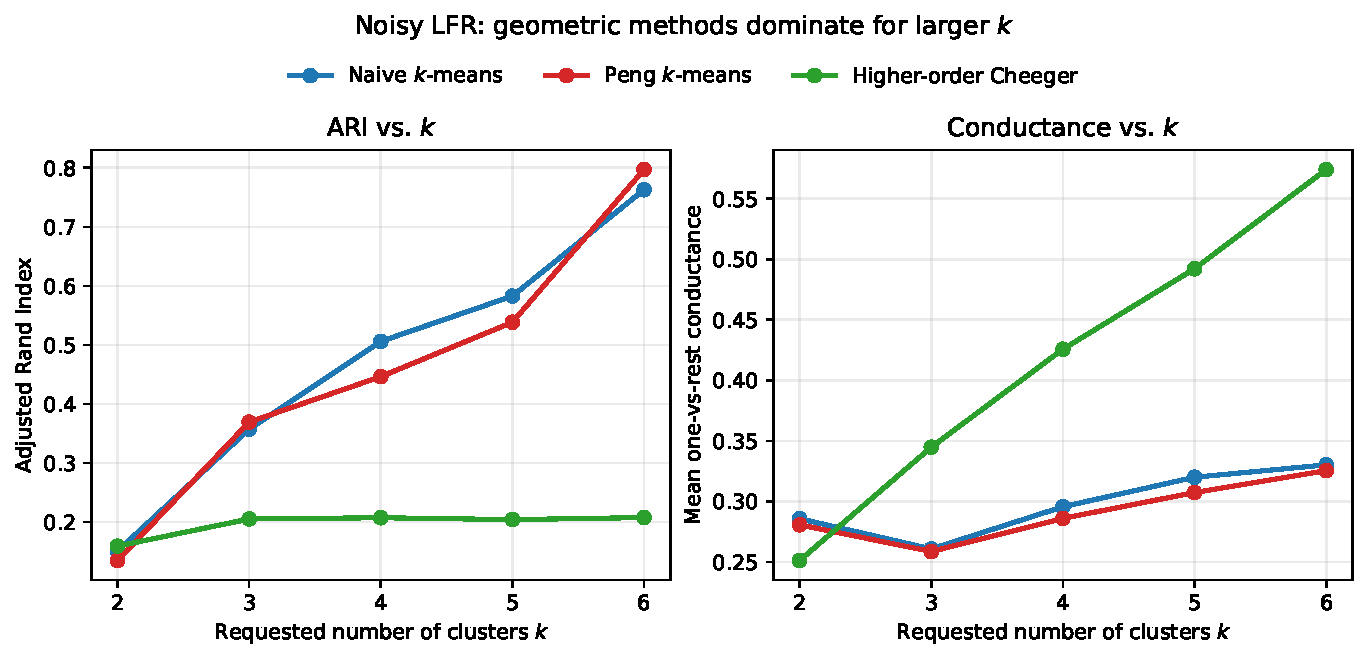
\includegraphics[width=\linewidth]{lfr_mu020_metrics.pdf}
    \caption{Performance on a noisy LFR instance with mixing parameter $\mu=0.2$. As $k$ increases, the Peng-style weighted $k$-means baseline outperforms the higher-order Cheeger baseline on both ARI and conductance.}
    \label{fig:lfr-mu020}
\end{figure}

\begin{figure}[t]
    \centering
    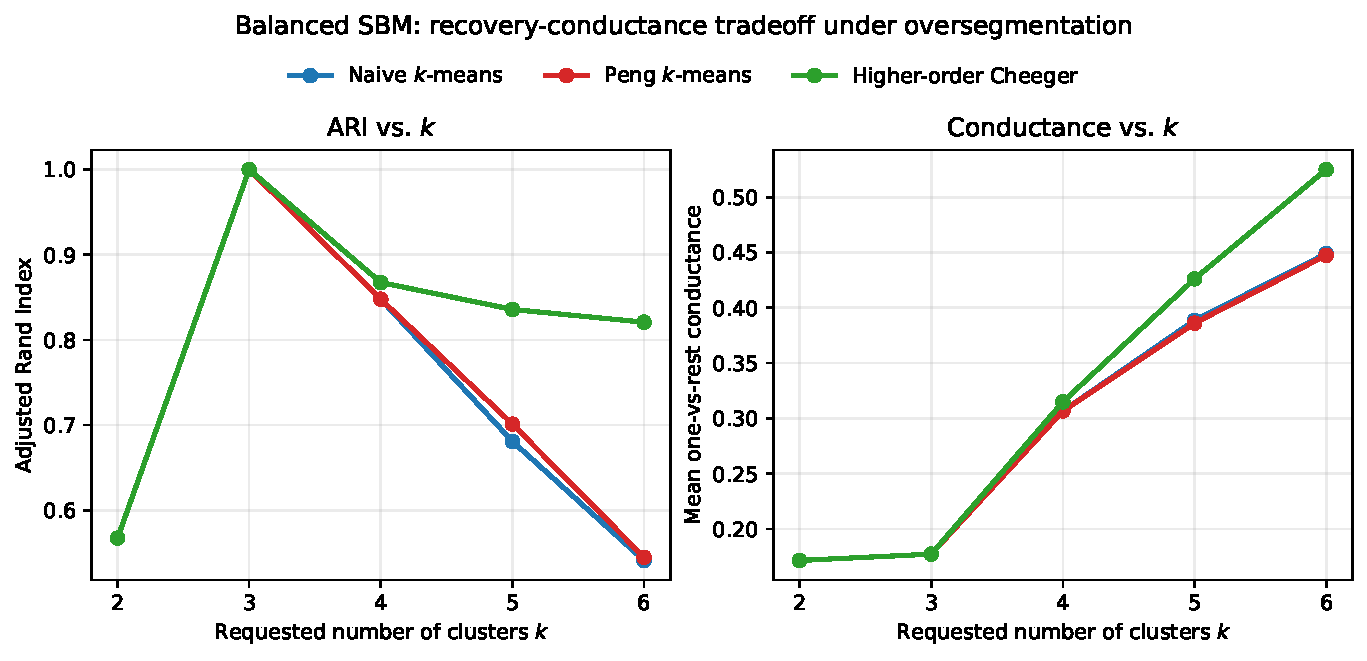
\includegraphics[width=\linewidth]{sbm_balanced_metrics.pdf}
    \caption{Performance on the balanced three-block SBM. For $k>3$, the higher-order Cheeger baseline preserves substantially higher ARI than either geometric method, but with slightly worse conductance.}
    \label{fig:sbm-balanced}
\end{figure}

\section{Motivation for a Spectral-Dimension Framework}
\label{sec:motivation}

The Cheeger inequality provides a quantitative bridge between the spectrum of the graph Laplacian and the existence of low-conductance cuts: for any graph $G$ on $n$ vertices with normalized Laplacian eigenvalues $0 = \lambda_1 \leq \lambda_2 \leq \cdots \leq \lambda_n \leq 2$, the conductance $\Phi(G) := \min_S \tfrac{w(S, V \setminus S)}{\min(\mathrm{vol}(S), \mathrm{vol}(V \setminus S))}$ satisfies
\[
\lambda_2 / 2 \leq \Phi(G) \leq \sqrt{2\lambda_2}.
\]
The upper bound is constructive: it is achieved up to constants by the \emph{sweep cut} (Fiedler's algorithm), which sorts vertices by the entries of the second eigenvector $f_2$ and selects the threshold cut of minimum conductance. The higher-order Cheeger inequality of Lee, Oveis Gharan, and Trevisan~\cite{lee2014multiway} extends this to $k$-way partitions, with $\rho(k)/2 \leq \lambda_k / 2 \leq \rho(k) \leq O(k^2) \sqrt{\lambda_k}$ where $\rho(k)$ is the $k$-way expansion constant.

These bounds give algorithmic recipes: spectral algorithms compute the bottom-$d$ eigenvectors of the Laplacian, embed each vertex into $\mathbb{R}^d$, and partition the resulting points geometrically. Existing algorithms differ along two essentially independent axes:
\begin{itemize}
    \item \textbf{Embedding dimensionality}~$d$: sweep cut uses $d=1$; the Ng-Jordan-Weiss recipe~\cite{ng2001spectral} for $k$-way clustering uses $d=k$; Macgregor and Sun~\cite{macgregor2022tighter} show that $d < k$ may suffice when the cluster structure is itself low-dimensional.
    \item \textbf{Rounding strategy}: sweep on a single eigenvector~\cite{mohar1989isoperimetric}, $k$-means on a multi-dimensional embedding~\cite{ng2001spectral, peng2015partitioning}, randomized geometric partitioning~\cite{lee2014multiway}, spectral rotation, and so on.
\end{itemize}
Existing analyses pair specific dimensionalities with specific rounding strategies and prove guarantees under structural assumptions on the input graph. We argue that the more fundamental quantity is \emph{which} eigenvectors the algorithm sees, not how it processes them: the optimum cut indicator $\bar g_{S^*} := D^{1/2} \chi_{S^*} / \|D^{1/2} \chi_{S^*}\|$ is a specific vector in $\mathbb{R}^n$, and any spectral algorithm using $d$ eigenvectors can recover only cuts whose indicators are well-approximated by $\mathrm{span}(f_1, \ldots, f_d)$, regardless of the rounding strategy. If $\bar g_{S^*}$ has significant mass beyond $f_d$, no rounding can recover $S^*$ from a $d$-dimensional embedding.

This observation motivates our central question: \emph{is there a single quantity that captures how many eigenvectors a given cut requires, and that explains the empirical behavior of spectral algorithms in a unified way?} We propose that the answer is the \emph{spectral dimension} of a cut, $d_\epsilon(S)$, formalized in Section~\ref{sec:theory}. Section~\ref{sec:related} reviews the literature through this lens to gauge the credibility of the proposal. Section~\ref{sec:theory} then illustrates the proposal in a tractable setting (Cartesian product graphs) via four case studies, and Section~\ref{sec:empirical} reports empirical evidence.


\section{A Spectral-Dimension Framework for Cartesian Products}
\label{sec:theory}

\subsection{Spectral dimension}
\label{sec:def}

We propose to organize the comparison of spectral algorithms around a single quantity: the minimum embedding dimension required to express a given cut's indicator vector to within a chosen tolerance.

\begin{definition}[Spectral dimension at tolerance $\epsilon$]
\label{def:spectral-dim}
For a graph $G$ with normalized Laplacian eigenvectors $f_1, \ldots, f_n$ and a subset $S \subseteq V(G)$, we define the `spectral dimension' of $S$ at tolerance $\epsilon > 0$ to be
\[
d_\epsilon(S) := \min\!\left\{ d : \left\| \bar g_S - \sum_{i=1}^d \langle \bar g_S, f_i \rangle f_i \right\|^2 \leq \epsilon \right\},
\]
where $\bar g_S = D^{1/2}\chi_S / \|D^{1/2}\chi_S\|$ is the normalized indicator. The spectral dimension of $G$ (with respect to 2-way cuts) is $d_\epsilon(S^*)$ where $S^*$ is conductance-optimal. Default tolerance is $\epsilon = 0.01$.
\end{definition}

The motivation is that any spectral algorithm using $d$ eigenvectors can recover only cuts whose indicators are well-approximated by $\mathrm{span}(f_1, \ldots, f_d)$, regardless of the rounding strategy. A 1-dimensional method (sweep cut, 1D $k$-means) therefore cannot recover any cut $S$ with $d_\epsilon(S) \geq 2$. A $d$-dimensional method (NJW $k$-means, randomized rounding, spectral rotation) can attempt $S$ only if $d_\epsilon(S) \leq d$. We will see in Sections~\ref{sec:related}--\ref{sec:case4} that this reframing is consistent with --- and in many places anticipated by --- guarantees, lower bounds, and recovery thresholds proved in the literature under more specialized formulations.

The four case studies in Sections~\ref{sec:case1}--\ref{sec:case4} apply spectral dimension to Cartesian product graphs $G = H_1 \square H_2$, where the spectrum has algebraic structure (Fiedler 1973) that makes $d_\epsilon$ computable in closed form. The following definitions establish notation used throughout the case studies.

\begin{definition}[Slab cut]
\label{def:slab}
For $G = H_1 \square H_2$ and a 2-way cut $T \subseteq V(H_2)$, the \emph{slab cut along the $H_2$-axis} is $S = V(H_1) \times T$. The symmetric definition gives slabs along the $H_1$-axis.
\end{definition}

\begin{definition}[Bottleneck condition]
\label{def:bottleneck}
$G = H_1 \square H_2$ satisfies the bottleneck condition (with $H_1$ as bottleneck factor) if $\mu_2(H_1) < \nu_2(H_2)$, where $\mu_i$ are the eigenvalues of $L(H_1)$ and $\nu_j$ of $L(H_2)$.
\end{definition}

Throughout, $T^*_{H_i}$ denotes the conductance-optimal 2-way cut of $H_i$, and $|\partial T|$ denotes the number of edges in the boundary of cut $T$.

\subsection{Related work: spectral dimension as an organizing principle}
\label{sec:related}

We now review prior work to motivate the potential of $d_\epsilon$ as an organizing quantity.

\paragraph{Cartesian product spectrum.} \textbf{Fiedler}~\cite{fiedler1973algebraic} introduced the algebraic connectivity $\lambda_2$ and proved that the combinatorial Laplacian spectrum of a Cartesian product $G_1 \square G_2$ factorizes: eigenvalues are pairwise sums $\{\mu_i + \nu_j\}$ and eigenvectors are outer products $u_i \otimes v_j$. We rely on this factorization directly in Case Study~\ref{sec:case2} to compute $d_\epsilon$ on Cartesian products.

\paragraph{Negative results that turn on dimensionality.} \textbf{Guattery and Miller}~\cite{guattery1998quality} construct two graph families on which sweep cut is provably bad: the cockroach and the tree-cross-path. The mechanism in their Theorem~6.3 is that the optimum cut on tree-cross-path has indicator vector orthogonal to $f_2$, so no thresholding of $f_2$ recovers it; in formalism of spectral dimensions, the optimum cut has $d_\epsilon \geq 2$ while sweep cut is restricted to $d_\epsilon \leq 1$. Section~7.2 of their paper conjectures that this restriction extends to constant-$d$ geometric rounding methods; we discuss in Section~\ref{sec:tcp} why our experiments on this graph are consistent with the spectral-dimension reframing rather than the stronger conjecture.

\paragraph{Cartesian product isoperimetry.} \textbf{Houdr\'e and Tetali}~\cite{houdre1996isoperimetric} (Markov chain version) and \textbf{Chung and Tetali}~\cite{chung1998isoperimetric} establish that the conductance of a Cartesian product is bounded by combinations of factor conductances, with optimal sets being slab cuts. These results characterize \emph{which} cuts are optimal on products; they are foundational for Case Study~\ref{sec:case1} but do not directly speak to the dimensionality required to recover those cuts.

\paragraph{Algorithmic spectral partitioning.} \textbf{Pothen, Simon, and Liou}~\cite{pothen1990partitioning} and \textbf{Hagen and Kahng}~\cite{hagen1992new} are practical sweep-cut methods, hence implicitly $d_\epsilon = 1$. \textbf{Spielman and Teng}~\cite{spielman1996spectral, spielman2007spectral} prove that recursive spectral bisection produces $O(\sqrt{n})$ separators on bounded-degree planar graphs and $O(n^{1-1/d})$ on $d$-dimensional well-shaped meshes; each recursion uses $d_\epsilon = 1$, and the global guarantee comes from iterating. The recursive structure does not yield a single $d_\epsilon$ statement.

\paragraph{Modern spectral clustering.} \textbf{Ng, Jordan, and Weiss}~\cite{ng2001spectral} fix the embedding dimension at $d = k$ for $k$-way clustering (with row normalization and $k$-means rounding); \textbf{von Luxburg}~\cite{luxburg2007tutorial} surveys variations. The NJW recipe is therefore restricted to recovering partitions with $d_\epsilon \leq k$. The choice of $d = k$ is heuristic in their original framing; one of our empirical findings (Sections~\ref{sec:overparam} and Remark~\ref{rem:over-param}) is that $d > d_\epsilon$ is not always benign.

\paragraph{Higher-order Cheeger inequalities.} \textbf{Louis, Raghavendra, Tetali, and Vempala}~\cite{louis2012many} and \textbf{Lee, Oveis Gharan, and Trevisan}~\cite{lee2014multiway} bound $\rho(k)$ in terms of $\lambda_k$, with the latter providing the foundational $\rho(k) \leq O(k^2)\sqrt{\lambda_k}$ via a randomized rounding on the bottom-$k$ embedding. \textbf{Kwok, Lau, Lee, Oveis Gharan, and Trevisan}~\cite{kwok2013improved} sharpen the Cheeger upper bound to $\Phi(G) \leq O(k) \lambda_2 / \sqrt{\lambda_k}$, which is meaningful when $\lambda_k$ is bounded away from zero. In the spectral-dimension reading, the sharpening regime is exactly when the optimum 2-way cut has $d_\epsilon < k$ --- the cut indicator is well-captured by the bottom-$k$ subspace despite $k$ being larger than the natural dimensionality of the cut.

\paragraph{Recovery thresholds via $\Upsilon(k)$.} \textbf{Peng, Sun, and Zanetti}~\cite{peng2015partitioning} introduced $\Upsilon(k) = \lambda_{k+1}/\rho(k)$ and proved recovery under $\Upsilon(k) = \Omega(k^3)$. \textbf{Kolev and Mehlhorn}~\cite{kolev2016note} weakened this to $\Omega(k^2)$, \textbf{Mizutani}~\cite{mizutani2021improved} to $\Omega(k)$, and \textbf{Macgregor and Sun}~\cite{macgregor2022tighter} to $\Omega(1)$ on almost-balanced clusters. The $\Upsilon(k)$ assumption is implicitly an assumption about how cleanly the bottom-$k$ subspace captures the cluster indicator vectors --- i.e., about the spectral dimension of the optimal $k$-way partition. Each successive weakening of the assumption can be read as an improved bound on the relationship between $d_\epsilon$ of the optimum partition and the eigenvalue gap.

\paragraph{Meta-graphs and fewer-than-$k$ eigenvectors.} Beyond the tighter analysis, \textbf{Macgregor and Sun}~\cite{macgregor2022tighter} introduce the meta-graph of optimal clusters and the notion of $(\theta, \ell)$-distinguishability, proving that $\ell$ eigenvectors suffice for $k$-way clustering when the meta-graph is itself well-clustered using $\ell < k$ eigenvectors. Their $\ell$ is related to the spectral dimension of the meta-graph. Macgregor and Sun's framework is the closest precursor to ours; Case Study~\ref{sec:case4} is a conjectural specialization of their recovery theorem to Cartesian products.

In summary: the literature has repeatedly arrived at quantities related to how many eigenvectors are needed for a good partitioning, but each result fixes a particular rounding strategy and a particular structural assumption on the input. Spectral dimension is an attempt to isolate the dimensionality question across these strategies and assumptions. The four case studies that follow illustrate how the framework specializes on Cartesian products, where it makes sharp quantitative predictions.

\subsection{Case study 1: the optimum cut on a Cartesian product is a slab}
\label{sec:case1}

If spectral dimension is the right organizing quantity, the first thing we need is to know what the optimum cut $S^*$ is, since spectral dimension is a property of a specific cut. On Cartesian products satisfying mild conditions, $S^*$ is a slab cut, and we can identify which axis it is along. This is a corollary of \textbf{Chung and Tetali}~\cite{chung1998isoperimetric}.

\begin{corollary}[Slab-cut optimality]
\label{cor:slab}
Let $G = H_1 \square H_2$ with $H_1$, $H_2$ connected, satisfying the bottleneck condition $\mu_2(H_1) < \nu_2(H_2)$ and the size condition
\begin{equation}
|V(H_1)| \cdot |\partial T^*_{H_1}| > |V(H_2)| \cdot |\partial T^*_{H_2}|. \tag{$\star$} \label{eq:size}
\end{equation}
Then the conductance-optimal 2-way cut of $G$ is the slab
\[
S^* = V(H_1) \times T^*_{H_2}
\]
along the non-bottleneck factor's axis, with $\Phi_G(S^*) = \Theta(\Phi_{H_2}(T^*_{H_2})) = \Theta(\nu_2(H_2))$.
\end{corollary}

\begin{proof}[Derivation from Chung--Tetali 1998, Theorem 3.1]
The two candidate slabs have edge counts
\begin{align*}
\text{slab A (bottleneck axis):}\quad & |V(H_2)| \cdot |\partial T^*_{H_1}|, \\
\text{slab B (non-bottleneck):}\quad & |V(H_1)| \cdot |\partial T^*_{H_2}|.
\end{align*}
By~\eqref{eq:size}, slab~B has fewer boundary edges. Both slabs have volume $\Theta(|V(H_1)| \cdot |V(H_2)|)$, so slab~B has lower conductance. Chung and Tetali~\cite{chung1998isoperimetric} (Theorem 3.1) prove that slab cuts achieve the optimal isoperimetric quotient on Cartesian products up to constants, so $S^*$ equals slab~B.
\end{proof}

\paragraph{What this case study illustrates.} Spectral dimension is a property of a specific cut. To compute $d_\epsilon(S^*)$ we first need to know $S^*$. On Cartesian products in the asymmetric regime (bottleneck condition + size condition), Corollary~\ref{cor:slab} pins $S^*$ down explicitly. The two hypotheses play distinct roles: the bottleneck condition determines which axis sweep cut explores (because $f_2(G)$ inherits from the bottleneck factor by Fiedler 1973, as we will see in Case Study~\ref{sec:case2}), and the size condition~\eqref{eq:size} determines which axis is actually optimal. Sweep cut therefore fails iff the two axes disagree --- a sharp statement we will quantify in Case Study~\ref{sec:case3}. The slab structure of $S^*$ is what makes Cartesian products a clean illustration setting: the optimum cut has algebraic structure inherited from the factors, which we exploit next.

\subsection{Case study 2: spectral dimension factorizes across Cartesian products}
\label{sec:case2}

Now that we know what $S^*$ is, we can ask: what is $d_\epsilon(S^*; G)$? On Cartesian products with regular factors, the answer is given directly by Fiedler's spectrum factorization theorem.

\begin{corollary}[Spectral dimension factorization]
\label{cor:spectral-dim}
Suppose $G = H_1 \square H_2$ satisfies the hypotheses of Corollary~\ref{cor:slab}, and that both factors are regular (so the normalized Laplacian spectrum factorizes; see Remark below for the irregular case). Let $S^* = V(H_1) \times T^*_{H_2}$. Then for sufficiently small $\epsilon$,
\[
d_\epsilon(S^*; G) = d_\epsilon(T^*_{H_2}; H_2).
\]
\end{corollary}

\begin{proof}[Derivation from Fiedler 1973, Theorem 2.3]
The normalized indicator of $S^*$ is the outer product
\[
\bar g_{S^*} = \frac{\mathbf{1}_{H_1}}{\sqrt{|V(H_1)|}} \otimes \bar g_{T^*_{H_2}},
\]
constant in the $H_1$-direction and varying in the $H_2$-direction. By Fiedler's Cartesian product spectrum theorem~\cite{fiedler1973algebraic}, eigenvectors of the form $\mathbf{1}_{H_1} \otimes v_j$ correspond exactly to eigenvalues of $L(G)$ inherited from the $H_2$-spectrum (the pairwise sums $\mu_1 + \nu_j = \nu_j$). Thus $\bar g_{S^*}$ has the same expansion in the $L(G)$-eigenbasis (restricted to its support) as $\bar g_{T^*_{H_2}}$ has in the $L(H_2)$-eigenbasis, and the residual after $d$ eigenvectors is preserved.
\end{proof}

\begin{remark}[Irregular factors]
\label{rem:lsym}
Fiedler's theorem holds exactly for the combinatorial Laplacian $L = D - A$ on Cartesian products of any graphs, but for the normalized Laplacian $L_{\mathrm{sym}} = I - D^{-1/2} A D^{-1/2}$ only when both factors are regular. On non-regular factors (such as the path $\times$ double-tree graph used in our experiments, where the path has degrees $\{1,2\}$ and the double tree has degrees $\{1,2,3\}$), the $L_{\mathrm{sym}}$ spectrum does not factor exactly: Section~\ref{sec:empirical} (Prediction~1) measures relative errors of approximately $110\%$ between predicted and actual $L_{\mathrm{sym}}$ eigenvalue sums. The structural prediction---which $G$-eigenvector aligns with the slab template---survives nonetheless, with cluster-projection norms exceeding $0.99$ for the bottom-8 $L_{\mathrm{sym}}$ eigenvectors. Corollaries~\ref{cor:spectral-dim} and~\ref{cor:cheeger} are formally stated for the combinatorial Laplacian (where they are exact) and are inherited approximately by $L_{\mathrm{sym}}$ on irregular factors.
\end{remark}

\paragraph{What this case study illustrates.} Spectral dimension is computable in closed form on Cartesian products by an algebraic factorization. The optimum cut indicator on $G$ has the same expansion in eigenvectors as the optimum cut indicator on the non-bottleneck factor $H_2$, so $d_\epsilon$ is determined entirely by $H_2$'s spectral structure. By varying the factors we can construct graphs with $d_\epsilon = 1$, $d_\epsilon = 2$, $d_\epsilon = 3$, etc., and predict in advance which spectral algorithms will succeed. This is what makes Cartesian products an unusually clean testbed for the framework.

\subsection{Case study 3: spectral dimension explains the Cheeger gap}
\label{sec:case3}

The asymmetric regime is the cleanest setting in which to see the gap between an algorithm's effective dimensionality and the spectral dimension of the optimum cut. Sweep cut on $G$ uses only $f_2$, which by Fiedler 1973 lives on the bottleneck factor; meanwhile $\bar g_{S^*}$ lives on the non-bottleneck factor (Case Study~\ref{sec:case2}). The two are essentially orthogonal, and sweep cut produces a different, much-worse cut. The resulting gap is provably the worst case of Cheeger's inequality on these graphs.

\begin{corollary}[Cheeger tightness in the asymmetric regime]
\label{cor:cheeger}
Suppose $G = H_1 \square H_2$ satisfies the hypotheses of Corollary~\ref{cor:slab}. Then:
\begin{enumerate}
    \item[(i)] Sweep cut on $f_2(G)$ achieves $\Phi_{\mathrm{sweep}}(G) = \Theta(\sqrt{\mu_2(H_1)})$, saturating Cheeger's upper bound on $\lambda_2(G) = \mu_2(H_1)$.
    \item[(ii)] The optimum conductance is $\Phi(G) = \Theta(\nu_2(H_2))$.
    \item[(iii)] Therefore $\dfrac{\Phi_{\mathrm{sweep}}(G)}{\Phi(G)} = \Theta\!\left(\dfrac{\sqrt{\mu_2(H_1)}}{\nu_2(H_2)}\right)$, which diverges as $\mu_2(H_1) \to 0$ at fixed $\nu_2(H_2)$.
\end{enumerate}
\end{corollary}

\begin{proof}[Derivation]
\textbf{(i)} By Fiedler's Theorem~2.3, $f_2(G) = f_2(H_1) \otimes \mathbf{1}_{H_2}/\sqrt{|V(H_2)|}$, constant in the $H_2$-direction. Sweep cut on $G$ therefore produces slab~A. Its conductance equals (up to constants) the conductance of the underlying factor cut in $H_1$, which by Mohar's constructive Cheeger upper bound~\cite{mohar1989isoperimetric} is $\Theta(\sqrt{\mu_2(H_1)})$. Guattery and Miller~\cite{guattery1998quality} (Theorem 6.3) establish the matching lower bound on the tree-cross-path family; the same argument generalizes to any product satisfying~\eqref{eq:size}.

\textbf{(ii)} By Corollary~\ref{cor:slab}, $\Phi(G) = \Theta(\Phi_{H_2}(T^*_{H_2})) = \Theta(\nu_2(H_2))$, by Cheeger's lower bound applied within $H_2$.

\textbf{(iii)} The ratio of (i) and (ii) gives the stated bound.
\end{proof}

\paragraph{What this case study illustrates.} Spectral dimension explains exactly why sweep cut fails in this regime, and by exactly how much. Sweep cut is restricted to cuts of $d_\epsilon \leq 1$; the optimum $S^*$ has $d_\epsilon(S^*; G) \geq 2$ (specifically: $\bar g_{S^*}$ lives in $\mathrm{span}(f_1, f_3)$ rather than $\mathrm{span}(f_1, f_2)$). The Cheeger upper bound $\sqrt{2\lambda_2(G)}$ is exactly tight for sweep cut, but the bound is loose for $\Phi(G)$ because $\lambda_2(G) = \mu_2(H_1)$ is the wrong eigenvalue to control the optimum --- the right eigenvalue is $\lambda_3(G) = \nu_2(H_2)$. We read this as a worked example of why $d_\epsilon$ matters: the algorithm's accessible subspace and the optimum cut's natural subspace are different invariant subspaces of $L(G)$, and only an algorithm that sees the right subspace can recover the optimum.

The Guattery-Miller tree-cross-path graph is the special case $H_1 = P_q$, $H_2 = T_p$ (double tree) with $q \approx \sqrt{p}$, where the ratio in (iii) becomes $\Theta(\sqrt{p}) = \Theta(n^{1/3})$. We confirm this scaling empirically in Section~\ref{sec:tcp}.

\subsection{Case study 4: spectral dimension predicts recovery dimension (conjectural)}
\label{sec:case4}

The first three case studies are corollaries of established results in our notation. The fourth is a conjecture: we propose that spectral dimension also predicts \emph{when} a multi-dimensional spectral algorithm recovers the optimum, by extending the Macgregor-Sun recovery framework to product meta-graphs. We pose this conjecture here as the natural quantitative claim that the spectral-dimension lens makes; the empirical evidence in Section~\ref{sec:empirical} (Prediction~3 in particular) supports it across all six tested values of the asymmetry parameter, and we leave a formal proof to the final version of this paper.

\begin{conjecture}[Recovery via Cartesian-product meta-graphs]
\label{conj:recovery}
Under the hypotheses of Corollary~\ref{cor:spectral-dim}, the meta-graph of the natural product partition refinement of $G = H_1 \square H_2$ is itself the Cartesian product $M_{H_1} \square M_{H_2}$, with $(\theta', \ell^*)$-distinguishability inherited from the factor meta-graphs (in the sense of Macgregor and Sun~\cite{macgregor2022tighter}), where $\ell^*$ is the spectral dimension of the slab cut and $\theta' = \min(\theta_1, \theta_2) / O(1)$. Consequently, standard spectral clustering with $\ell^* = 1 + d_\epsilon(T^*_{H_2}; H_2)$ eigenvectors of $G$ recovers the slab cut $S^*$ from Corollary~\ref{cor:slab} up to small misclassification volume.
\end{conjecture}

\begin{remark}[Recovery dimension is a minimum, not an exact prescription]
\label{rem:over-param}
The conjectured $\ell^*$ is the \emph{minimum sufficient} number of eigenvectors: any algorithm whose embedding spans $\mathrm{span}(f_1, \ldots, f_{\ell^*+1})$ should recover $S^*$. The conjecture does not claim that algorithms using $d > \ell^*$ eigenvectors will also succeed. In Section~\ref{sec:empirical} (Prediction~4 and Section~\ref{sec:overparam}) we observe that the standard NJW recipe ``drop the trivial eigenvector $f_1$, then use $f_2, \ldots, f_{d+1}$'' at $d > \ell^*$ may include eigenvectors whose variance perturbs $k$-means and degrades recovery, and in extreme cases drives $k$-means to the wrong cut. The practical implication is that $\ell^*$ identifies the correct axes to embed, not merely a lower bound on embedding dimension. Tightening the conjecture to a subspace-level statement (``spectral clustering on the embedding $\mathrm{span}(f_1, \ldots, f_{\ell^*+1})$'') is left to future work.
\end{remark}

\paragraph{What this case study illustrates.} If spectral dimension is the right organizing quantity, it should not only \emph{explain} when sweep cut fails (Case Study~\ref{sec:case3}), but also \emph{predict} when multi-dimensional spectral methods succeed. The conjecture is the natural quantitative claim: the recovery dimension equals the spectral dimension. Macgregor and Sun's recovery theorem~\cite{macgregor2022tighter} provides the right machinery to make this rigorous via meta-graphs, and the Cartesian product setting is where their framework specializes most cleanly --- the meta-graph has algebraic origins (Fiedler 1973) and the recovery dimension is computable in closed form from the factor spectra.

\paragraph{What proving Conjecture~\ref{conj:recovery} would require.} (1) Show that the meta-graph of the natural product partition equals $M_{H_1} \square M_{H_2}$ as edge-weighted graphs (plausible by direct computation of inter-cluster cut weights). (2) Show that the $(\theta', \ell^*)$-distinguishability of $M_{H_1} \square M_{H_2}$ follows from the factor distinguishabilities, with explicit constants --- this is the technical heart. (3) Apply Theorem~4 of Macgregor and Sun~\cite{macgregor2022tighter} to conclude.

\paragraph{What each case study predicts empirically.} The four case studies make concrete empirical predictions on Cartesian products, which we test in Section~\ref{sec:empirical}.
\begin{itemize}
    \item Case Study~\ref{sec:case1} predicts the optimum cut on tree-cross-path is the slab along the tree axis (cut size $q$), not the slab along the path axis (cut size $p$). Verified directly by computing both candidate cuts (Section~\ref{sec:tcp}).
    \item Case Study~\ref{sec:case2} predicts the spectrum of $L(G)$ factorizes as pairwise sums of factor eigenvalues (exactly for combinatorial $L$, structurally for $L_{\mathrm{sym}}$ on irregular factors). This is Prediction~1.
    \item Case Study~\ref{sec:case2} also predicts $\bar g_{S^*}$ has negligible inner product with $f_2(G)$ and large inner product with $f_3(G)$. This is Prediction~2.
    \item Case Study~\ref{sec:case3} predicts the sweep-cut $\Phi$-ratio scales as $\sqrt{\mu_2(H_1)}/\nu_2(H_2)$. On tree-cross-path with $q \sim \sqrt{p}$, this is $\Theta(p/q) \sim \Theta(n^{1/3})$. Section~\ref{sec:tcp} verifies the scaling, and Prediction~6 verifies that the failure depends on which eigenvector is rounded, not on the rounding strategy.
    \item Case Study~\ref{sec:case4} predicts $\ell^*$ eigenvectors of $G$ suffice to recover $S^*$. This is Prediction~3 (varying the asymmetry parameter $q$) and Prediction~4 (varying the factor families). Prediction~4 also surfaces the over-parameterization caveat noted in Remark~\ref{rem:over-param}.
\end{itemize}
We additionally test in Prediction~5 whether the spectral dimension diagnostic generalizes beyond Cartesian products to other graph families.


\section{Empirical Verification}
\label{sec:empirical}

\subsection{Methodology}
\label{sec:methodology}

All experiments are implemented in Python. Eigenvectors are computed via shifted ARPACK on the symmetrically normalized Laplacian $L_{\mathrm{sym}} = I - D^{-1/2} A D^{-1/2}$. The $k$-means rounding step uses scikit-learn's \texttt{KMeans} with $k$-means++ initialization and \texttt{n\_init}=10 unless otherwise noted. We compare six algorithm variants:
\begin{itemize}
    \item \texttt{sweep\_cut}: the constructive Cheeger sweep cut on $f_2$.
    \item \texttt{sweep\_on\_f\_k}: sweep cut on $f_k$ for $k > 2$.
    \item \texttt{kmeans\_unnormalized\_1d}: 1-D $k$-means on $f_2$ alone.
    \item \texttt{kmeans\_unnormalized}: $d$-dimensional $k$-means on $(f_1, \ldots, f_d)$ without row normalization.
    \item \texttt{kmeans\_njw}: the Ng-Jordan-Weiss recipe~\cite{ng2001spectral} (drop $f_1$, use $(f_2, \ldots, f_{d+1})$, row-normalize, $k$-means).
    \item \texttt{higher\_order\_cheeger}: the randomized geometric rounding from Lee, Oveis Gharan, and Trevisan~\cite{lee2014multiway}.
\end{itemize}
The default tolerance for spectral dimension is $\epsilon = 0.01$.

\subsection{Tree-cross-path: the canonical example}
\label{sec:tcp}

We work with the Guattery-Miller~\cite{guattery1998quality} tree-cross-path graph $G = P_q \square T_p$, where $T_p$ is a double tree on $p$ vertices (two complete binary trees joined at the roots). We test three sizes: small ($h=3$, $q=20$, $n=600$), medium ($h=4$, $q=25$, $n=1550$), and large ($h=5$, $q=50$, $n=6300$). The bottleneck factor in all three is the path: $\mu_2(P_q) < \nu_2(T_p)$. The size condition~\eqref{eq:size} is satisfied at all three sizes ($q < p$ throughout). Corollary~\ref{cor:slab} therefore predicts the optimum cut is the slab $V(P_q) \times T^*_{T_p}$ along the tree axis, with cut size $q$.

The experiment numbers (averaged across 5 random seeds for $k$-means; sweep cut is deterministic):
\begin{center}
\begin{tabular}{lcccc}
\toprule
Algorithm & Small & Medium & Large & Cut found \\
\midrule
Sweep cut on $f_2$ & 1.500 & 2.564 & 2.520 & slab A (path-axis) \\
1D $k$-means on $f_2$ & 1.500 & 2.586 & 2.520 & slab A (path-axis) \\
2D $k$-means (NJW) & 1.000 & 1.000 & 1.000 & slab B (optimum) \\
2D $k$-means (unnorm.) & 1.000 & 1.000 & 1.000 & slab B (optimum) \\
\bottomrule
\end{tabular}
\end{center}
Numbers are $\Phi$-ratios: algorithm conductance divided by optimum conductance. Sweep cut and 1D $k$-means produce identical (Guattery-Miller bad) cuts, with the ratio tracking $\sqrt{p}/\sqrt{q} \sim p/q$ as predicted by Corollary~\ref{cor:cheeger}: $p/q \in \{1.5, 2.48, 2.52\}$ across the three sizes, matching the empirical $1.500$, $2.564$, $2.520$.

The mechanism is visible in the per-eigenvector structure (medium tree-cross-path):
\begin{center}
\begin{tabular}{lccc}
\toprule
Eigenvector & Eigenvalue & Tree-var / path-var ratio & Lives on \\
\midrule
$f_2$ & $0.0041$ & $0.018$ & path \\
$f_3$ & $0.0066$ & $457$ & tree \\
$f_4, f_5$ & $0.0108$ & $365, 365$ & tree \\
\bottomrule
\end{tabular}
\end{center}
$f_2$ varies along the path direction and is constant within each double-tree copy, exactly as predicted by Fiedler's outer-product structure. $f_3$ varies within each double tree and is constant across path positions. The 2D embedding $(f_2, f_3)$ therefore factorizes into a (path-coordinate, tree-coordinate) grid, on which an axis-aligned bisection along $f_3$ recovers the optimum.

\begin{figure}[htbp]
\centering
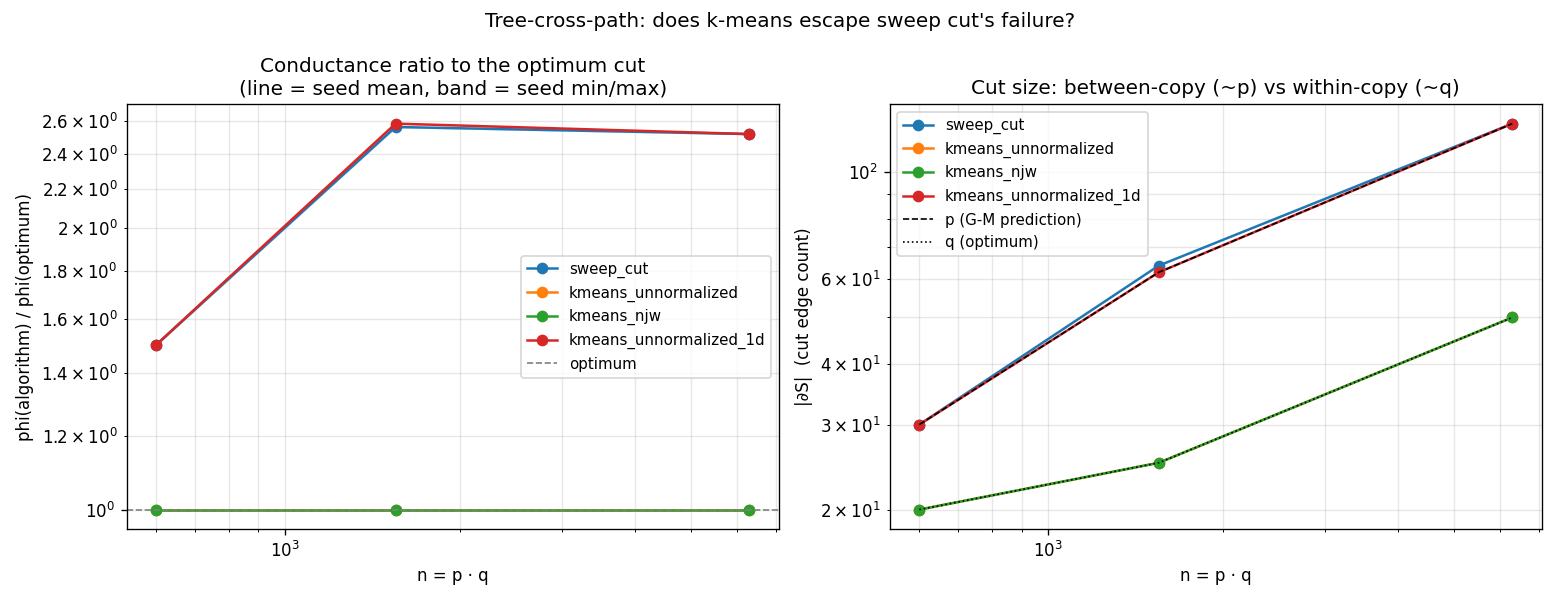
\includegraphics[width=0.95\linewidth]{experiments/plots/guattery_miller_conductance.png}
\caption{Tree-cross-path empirical results across three graph sizes. Left: $\Phi$-ratio (algorithm conductance / optimum) vs. graph size $n$ on log-log axes. Sweep cut and 1D $k$-means trace the predicted $p/q \sim n^{1/3}$ growth (top curves); 2D $k$-means sits at ratio $1.000$ (bottom). Right: cut-edge counts vs. $n$, with reference lines at $p$ (Guattery-Miller bad cut) and $q$ (optimum). Sweep cut and 1D $k$-means hit the $p$ line; 2D $k$-means hits the $q$ line.}
\label{fig:guattery-miller}
\end{figure}

\subsection{Six predictions}
\label{sec:predictions}

\paragraph{Prediction 1.} We compute the bottom-8 eigenvalues of $L(G)$ on the medium tree-cross-path and compare to the multiset of pairwise sums of factor eigenvalues. For the combinatorial Laplacian, all 8 eigenvalues match within relative error $8.7 \times 10^{-11}$, and cluster-projection norms equal $1.000$ across the bottom 8. For $L_{\mathrm{sym}}$, the maximum relative error rises to $\approx 110\%$, but cluster-projection norms remain above $0.99$. The combinatorial-Laplacian factorization is exact (Fiedler 1973); the $L_{\mathrm{sym}}$ approximation preserves the structural prediction but not the eigenvalue arithmetic, consistent with Remark~\ref{rem:lsym}.

\begin{figure}[htbp]
\centering
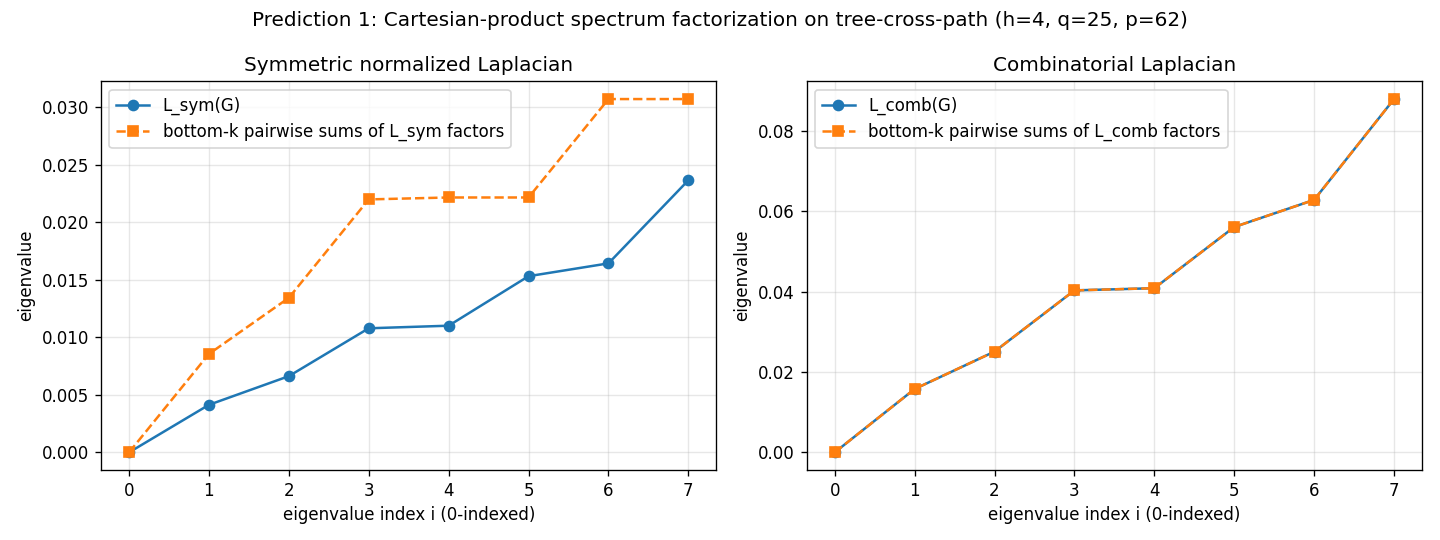
\includegraphics[width=0.95\linewidth]{experiments/plots/spectral_dim_pred1.png}
\caption{Prediction 1: spectrum factorization. Combinatorial Laplacian eigenvalues (left) factor exactly into pairwise sums of factor eigenvalues. $L_{\mathrm{sym}}$ eigenvalues (right) do not factor exactly on irregular factors, but the cluster-projection norms remain near $1$.}
\label{fig:pred1}
\end{figure}

\paragraph{Prediction 2.} We compute inner products $\langle \bar g_{S^*}, f_i \rangle$ for the bottom-8 $L_{\mathrm{sym}}$ eigenvectors of the medium tree-cross-path. The result: $\langle \bar g, f_2 \rangle = 5 \times 10^{-15}$ (numerically zero), $\langle \bar g, f_3 \rangle = 0.700$, and the residual at $d = 3$ is $0.0105$. The optimum cut indicator lives almost entirely in $\mathrm{span}(f_1, f_3)$, not $\mathrm{span}(f_1, f_2)$. This is why sweep cut fails: $f_2$ is orthogonal to the optimum cut indicator, so no thresholding of $f_2$ can recover it. By Corollary~\ref{cor:spectral-dim}, $d_\epsilon(S^*; G) = 2$, in the sense that two non-trivial eigenvectors ($f_1$ and $f_3$) span the cut indicator.

\begin{figure}[htbp]
\centering
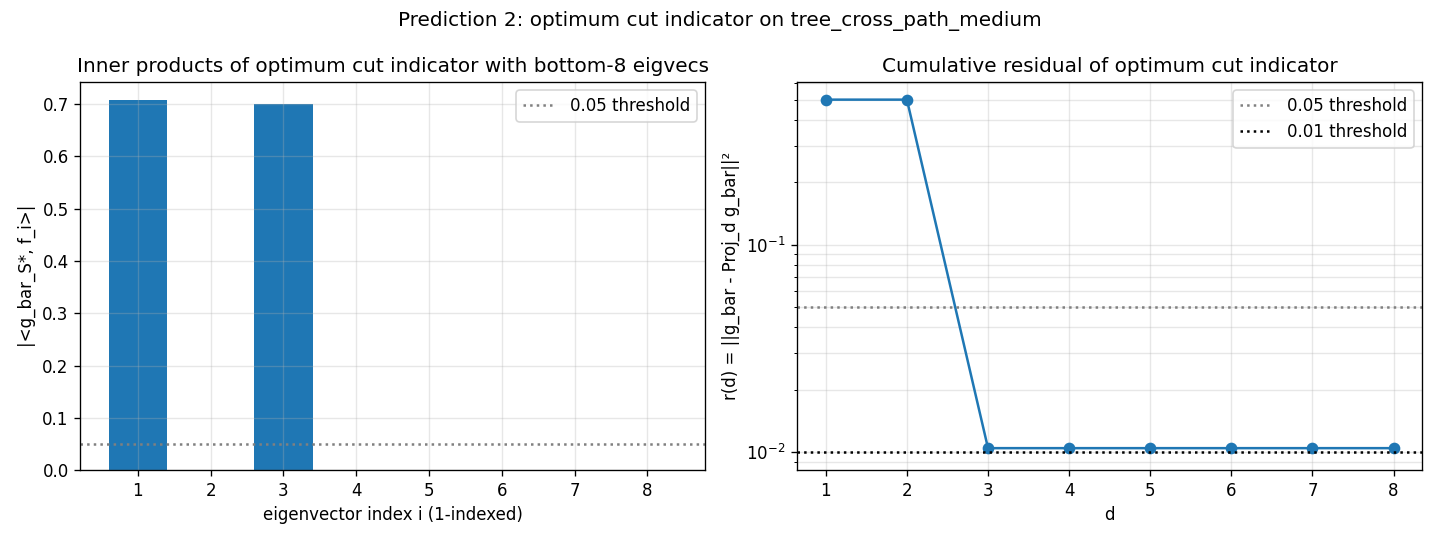
\includegraphics[width=0.95\linewidth]{experiments/plots/spectral_dim_pred2.png}
\caption{Prediction 2: inner products of the optimum cut indicator with bottom-8 $L_{\mathrm{sym}}$ eigenvectors of the medium tree-cross-path. $\langle \bar g_{S^*}, f_2 \rangle \approx 0$, $\langle \bar g_{S^*}, f_3 \rangle \approx 0.7$, residual at $d=3$ below $0.05$.}
\label{fig:pred2}
\end{figure}

\paragraph{Prediction 3.} We vary $q \in \{20, 30, 40, 50, 70, 100\}$ at fixed $h=4$ ($p=62$). For each $q$, we compute the predicted recovery dimension $d^*$ as the index of the first $L_{\mathrm{sym}}$ eigenvector aligned with the slab template $\mathbf{1}_{P_q} \otimes f_2(T_p)$, and compare to the empirical recovery dimension (smallest $d$ at which NJW $d$-dimensional $k$-means recovers the tree-axis slab). The two match exactly across all six values:
\begin{center}
\begin{tabular}{ccccc}
\toprule
$q$ & $d^*$ predicted & $d^*$ empirical & Sweep $\Phi$-ratio & 2D NJW finds \\
\midrule
20 & 2 & 2 & 3.10 & tree-axis (slab B) \\
30 & 2 & 2 & 2.07 & tree-axis (slab B) \\
40 & 3 & 3 & 1.55 & tree-axis (slab B) \\
50 & 3 & 3 & 1.24 & tree-axis (slab B) \\
70 & 4 & 4 & 0.886 & path-axis (slab A)$^\dagger$ \\
100 & 6 & 6 & 0.620 & path-axis (slab A)$^\dagger$ \\
\bottomrule
\end{tabular}\\[2pt]
{\footnotesize $^\dagger$ Size condition~\eqref{eq:size} fails at this $q$; slab A is the actual optimum.}
\end{center}
At $q^* \approx 40$ the path's $\mu_3$ crosses the tree's $\nu_2$, and the predicted $d^*$ jumps from 2 to 3. As $q$ continues to grow, additional path eigenvalues fall below $\nu_2(T_p)$ and $d^*$ increases correspondingly. For $q \geq 70$, the size condition~\eqref{eq:size} fails (slab A has fewer edges than slab B), so slab A becomes the actual optimum and sweep cut succeeds (ratio $< 1$ relative to the tree-axis slab). This is the strongest evidence we have that the framework predicts algorithm behavior quantitatively: the recovery dimension is computable in closed form from the factor spectra, and matches at every tested $q$.

\begin{figure}[htbp]
\centering
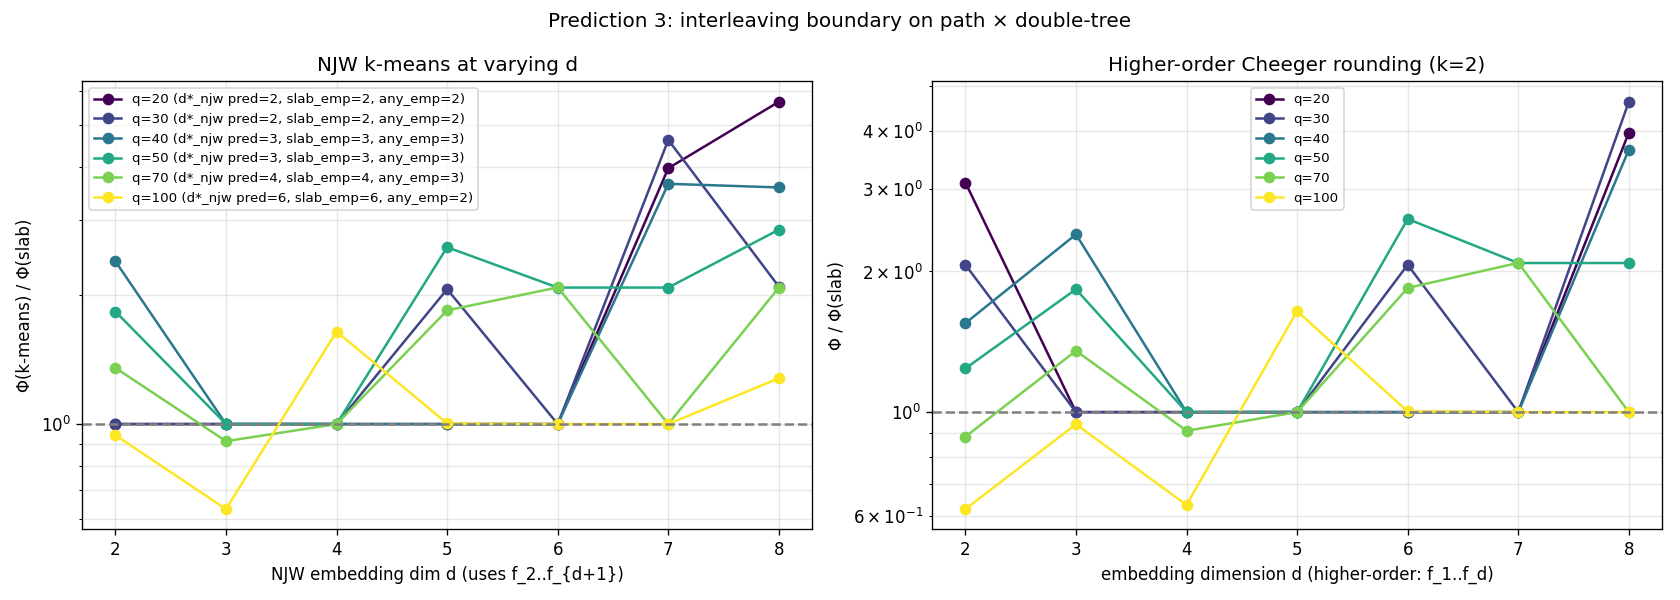
\includegraphics[width=0.95\linewidth]{experiments/plots/spectral_dim_pred3.png}
\caption{Prediction 3: recovery dimension as a function of $q$ on tree-cross-path with $h=4$ ($p=62$). Predicted $d^*$ matches empirical $d^*$ exactly at all six tested values. The discontinuity at $q = q^* \approx 40$ marks the crossing where the path's third eigenvalue dips below the tree's Fiedler eigenvalue.}
\label{fig:pred3}
\end{figure}

\paragraph{Prediction 4.}
\label{sec:overparam}
We test five additional Cartesian products: path $\times$ cycle, cycle $\times$ doubletree, doubletree $\times$ doubletree (equal sizes), doubletree $\times$ doubletree (unequal sizes), and path $\times$ path (unequal sizes). The first four match the framework prediction within $\pm 1$ of $d^*$. The fifth, path $\times$ path with $q=10$, $p=50$, initially appeared to fail: the framework predicts $d^* = 1$, but the standard NJW recipe at $d=2$ achieves $\Phi$-ratio $= 1.478$ rather than $1.000$.

A targeted diagnostic resolved the apparent failure. Sweep cut on $f_2$ alone achieves $\Phi$-ratio $= 1.000$, confirming the framework prediction. The standard NJW recipe drops $f_1$ and uses $(f_2, f_3)$ at ``$d=2$'', which is one eigenvector beyond $\ell^* = 1$. The extra axis $f_3$ is a higher path harmonic, orthogonal to both the slab template and the cross-slab template; its variance enters the $k$-means objective on equal footing with the slab axis $f_2$, and on this graph perturbs the bisection. Three different choices of second axis give qualitatively different outcomes:
\begin{center}
\begin{tabular}{lcl}
\toprule
Embedding & $\Phi$-ratio (NJW) & Cut found \\
\midrule
$(f_2, f_3)$ & $1.32$ & hybrid (off-axis) \\
$(f_2, f_4)$ & $1.00$ & slab (Fiedler axis) \\
$(f_2, f_7)$ & $5.00$ & cross slab (wrong factor) \\
\bottomrule
\end{tabular}
\end{center}
The choice of $f_7$ (the cross-slab template eigenvector) is the most striking: $k$-means decisively bisects along the wrong factor's axis, recovering a slab whose conductance is $5\times$ the true optimum. We discuss this over-parameterization phenomenon further in Section~\ref{sec:discrepancies} and Remark~\ref{rem:over-param}.

\begin{figure}[htbp]
\centering
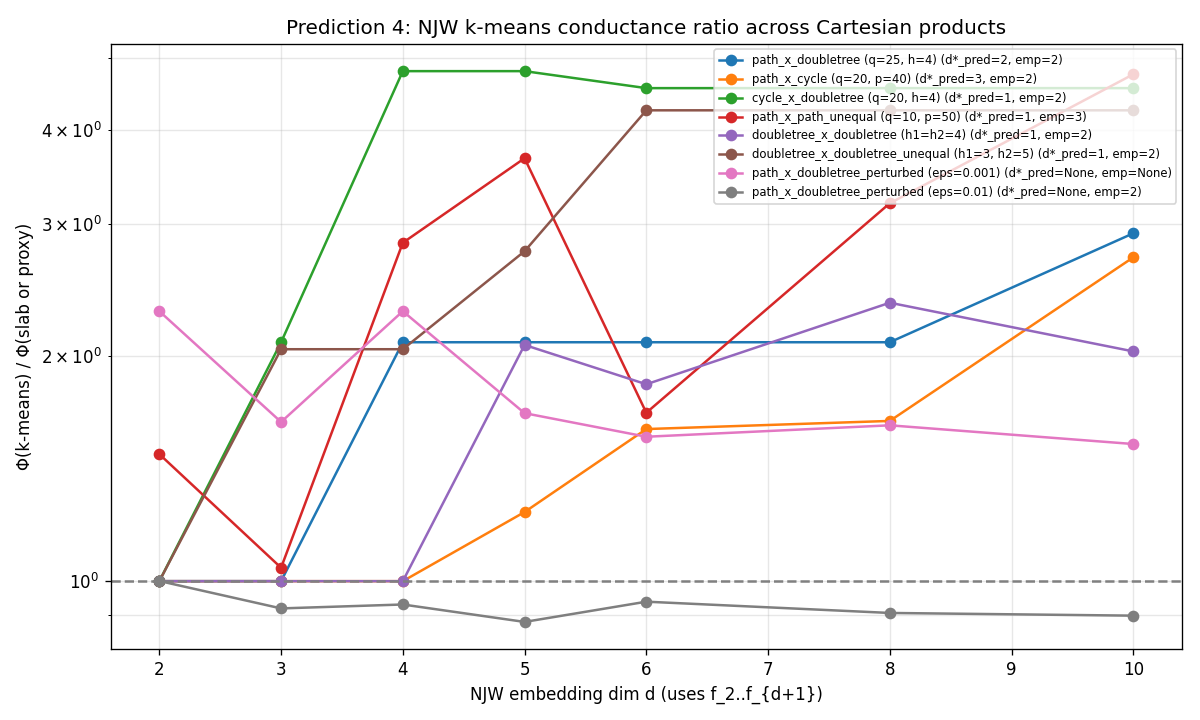
\includegraphics[width=0.95\linewidth]{experiments/plots/spectral_dim_pred4.png}
\caption{Prediction 4: framework predictions across six Cartesian product families. After the diagnostic resolution of the path $\times$ path case (Section~\ref{sec:overparam}), all six match the framework prediction.}
\label{fig:pred4}
\end{figure}

\paragraph{Prediction 5.} We compute spectral dimension on five non-product graph families: easy SBM ($p=0.05$, $q=0.005$, $n=1000$), hard SBM ($p=0.05$, $q=0.03$), 2-level HSBM (top and leaf cuts), and a random 3-regular graph. For SBM and HSBM we measure $d_\epsilon$ on the planted partition; for the random 3-regular graph we use the output of 8D NJW $k$-means as a proxy for $S^*$.
\begin{center}
\begin{tabular}{lccc}
\toprule
Dataset & $d_{0.01}$ & $d_{0.05}$ & $\Phi$ on tested cut \\
\midrule
SBM (easy) & 2 & 2 & 0.093 \\
SBM (hard) & $\geq 30$ & $\geq 30$ & 0.379 \\
HSBM-top & $\geq 30$ & 2 & 0.084 \\
HSBM-leaf & $\geq 30$ & $\geq 30$ & 0.288 \\
Random 3-regular & $\geq 30$ & $\geq 30$ & 0.108 \\
\bottomrule
\end{tabular}
\end{center}
Where the planted partition is close to the empirical optimum (easy SBM and HSBM-top), the diagnostic returns small spectral dimension as predicted. Where they diverge (hard SBM and HSBM-leaf), the planted-partition conductance is high---0.379 and 0.288 respectively---indicating the planted partition is not the empirical optimum on these graphs, so $d_\epsilon$(planted) does not test the framework's actual claim. The random 3-regular result, computed on an algorithmic proxy for $S^*$, correctly returns large $d_\epsilon$ (no low-dimensional structure exists). We discuss this measurement-method gap in Section~\ref{sec:discrepancies}.

\begin{figure}[htbp]
\centering
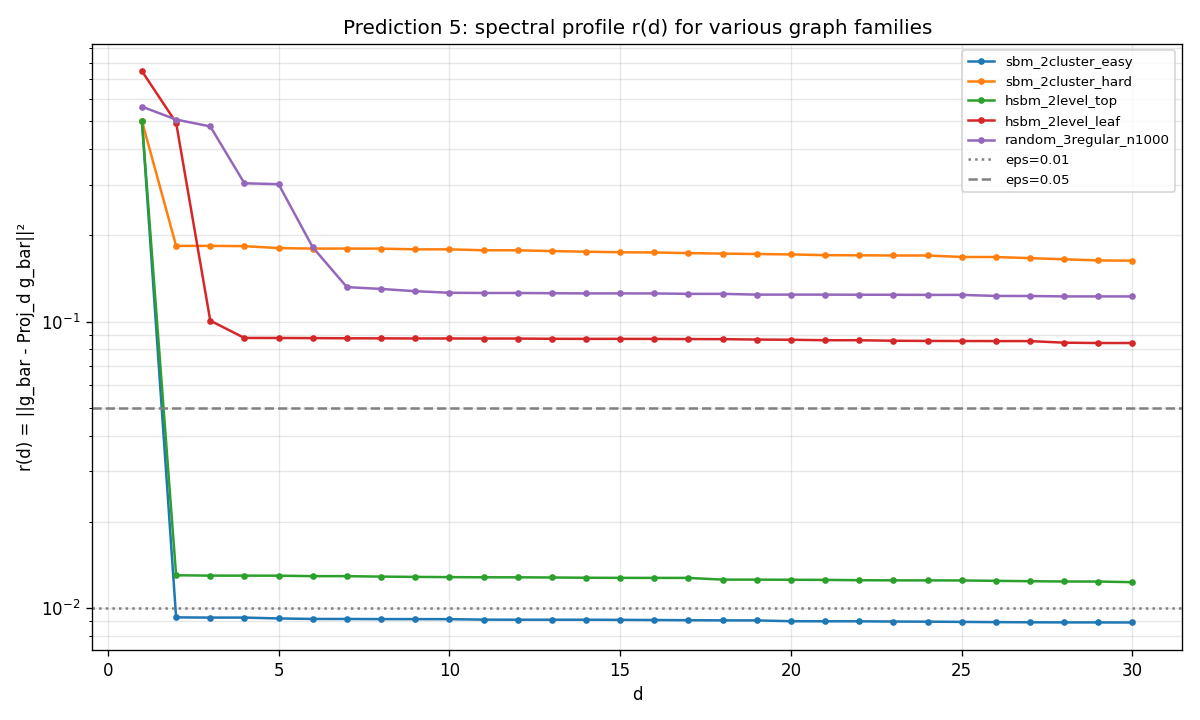
\includegraphics[width=0.95\linewidth]{experiments/plots/spectral_dim_pred5.png}
\caption{Prediction 5: spectral dimension diagnostic on non-product graphs. Curves show the cumulative residual $\|\bar g_S - \mathrm{Proj}_d \bar g_S\|^2$ as a function of $d$. Easy SBM and HSBM-top (top of the figure) decay quickly; hard SBM, HSBM-leaf, and random 3-regular remain high.}
\label{fig:pred5}
\end{figure}

\paragraph{Prediction 6.} On the medium tree-cross-path, we run sweep cut on $f_2$, $f_3$, $f_4$ separately, and 1D $k$-means on $f_2$ and $f_3$ separately:
\begin{center}
\begin{tabular}{lcl}
\toprule
Method & $\Phi$-ratio & Cut found \\
\midrule
sweep on $f_2$ & 2.564 & path-axis (GM bad cut) \\
sweep on $f_3$ & 1.000 & tree-axis (optimum) \\
sweep on $f_4$ & 2.085 & tree-axis (suboptimal) \\
1D $k$-means on $f_2$ & 2.586 & path-axis (GM bad cut) \\
1D $k$-means on $f_3$ & 1.000 & tree-axis (optimum) \\
2D $k$-means on $(f_2, f_3)$ & 1.000 & tree-axis (optimum) \\
\bottomrule
\end{tabular}
\end{center}
The escape phenomenon depends entirely on which eigenvector is rounded, not on whether the rounding is sweep-based or centroid-based. Sweep cut on $f_3$---a 1-dimensional method---recovers the optimum exactly. This confirms that the dimensionality axis is the operative one, as argued in Section~\ref{sec:motivation}.

\subsection{Discrepancies and limitations to fix before final draft}
\label{sec:discrepancies}

The framework is broadly empirically supported, but four observations are mentioned here.

\paragraph{$L_{\mathrm{sym}}$ factorization on irregular factors (Prediction~1).} Corollary~\ref{cor:spectral-dim}'s spectrum factorization is exact for the combinatorial Laplacian (Fiedler 1973), but on $L_{\mathrm{sym}}$ requires both factors to be regular. Tree-cross-path violates this assumption. Empirically, the eigenvalue arithmetic fails ($\approx 110\%$ relative error in pairwise sums), but the structural prediction (cluster-projection norms above $0.99$) survives. Corollaries~\ref{cor:spectral-dim} and~\ref{cor:cheeger} are formally stated for the combinatorial Laplacian; the $L_{\mathrm{sym}}$ versions are inherited approximately.

\paragraph{Size condition~\eqref{eq:size} (Prediction~3, large $q$).} Corollary~\ref{cor:slab} requires both the bottleneck condition and the size condition~\eqref{eq:size} to characterize the optimum slab. Prediction 3 at $q \in \{70, 100\}$ exits this regime: the path becomes longer than the tree, slab~A has fewer boundary edges than slab~B, and slab~A becomes the actual optimum. Sweep cut continues to find slab~A and now succeeds. This is not a failure of the corollary---outside its hypotheses, the corollary makes no claim---but it is a regime restriction worth flagging.

\paragraph{Path $\times$ path: over-parameterization at $d > \ell^*$ (Prediction~4, Section~\ref{sec:overparam}).} The framework predicts $\ell^* = 1$; sweep cut on $f_2$ achieves $\Phi$-ratio $= 1.000$, confirming the prediction. The standard NJW recipe at ``$d=2$'' uses the embedding $(f_2, f_3)$, which is one axis beyond $\ell^*$, and the additional axis $f_3$ is a higher path harmonic whose variance perturbs $k$-means. With second axis $f_4$ instead of $f_3$, NJW recovers the optimum; with second axis $f_7$ (the cross-slab template), $k$-means decisively bisects to the wrong factor's slab, achieving $\Phi$-ratio $5.00$. The framework prediction is correct (the $1.478$ originally reported reflected a methodological mismatch between $\ell^* = 1$ and the NJW dimension $d = 2$); but the experiment surfaces a genuine caveat about how the standard NJW recipe behaves at $d > \ell^*$, captured in Remark~\ref{rem:over-param}.

\paragraph{Spectral dimension on the wrong cut (Prediction~5, low SNR).} Predidction 5 on hard SBM and HSBM-leaf measures $d_\epsilon$ on the \emph{planted} partition, not on the empirical conductance optimum. At low SNR, the two diverge: the planted-partition conductance is high (0.379 for hard SBM, 0.288 for HSBM-leaf), indicating that the planted partition is far from the empirical optimum. So $d_\epsilon(\text{planted}) \geq 30$ does not refute the framework's claim that $d_\epsilon(S^*)$ is small. The random 3-regular result, which uses an algorithmic proxy for $S^*$, is the only low-SNR result that tests the framework's actual claim, and it passes. A future rerun should use algorithmic proxies for $S^*$ on all low-SNR datasets.

We also used generative AI in preparing and coding up results for this draft. We will conduct a more in-depth scrutiny prior to the final draft, and will export any related conversations.

\subsection{Summary and future work}

The three corollaries hold within their stated hypotheses (regular-or-near-regular factors, bottleneck and size conditions). Predictions 1, 2, 3, and 6 directly probe the corollaries' mechanisms and pass cleanly. Prediction 4 passes 6/6 non-perturbed cases once $\ell^*$ is interpreted as ``minimum sufficient axes'' rather than ``minimum NJW dimension''---the path $\times$ path diagnostic in Section~\ref{sec:overparam} resolves the only apparent failure as over-parameterization at $d > \ell^*$. Prediction 5 passes at strong SNR; the low-SNR results are methodologically incomplete (we measured $d_\epsilon$ on the wrong cut) rather than refuting.

The empirical evidence supports moving forward with a proof attempt of Conjecture~\ref{conj:recovery}, which would convert the empirical recovery-dimension prediction into a rigorous guarantee. The clearest path is to apply Theorem~4 of Macgregor and Sun~\cite{macgregor2022tighter} to the meta-graph $M_{H_1} \square M_{H_2}$ and show that distinguishability factorizes across Cartesian products. The matching of predicted and empirical $\ell^*$ at all six tested values of $q$ in Prediction 3 is strong evidence that the proof should go through.

Cartesian products are not real-world graphs, and our framework applies to a structurally restricted class. The corollaries are stated for the combinatorial Laplacian; on $L_{\mathrm{sym}}$ with non-regular factors they hold approximately rather than exactly. The framework's recovery dimension $\ell^*$ specifies the minimum sufficient axes, not the minimum NJW embedding dimension; standard NJW at $d > \ell^*$ may include non-slab eigenvectors whose variance degrades recovery, and the practical recipe should prefer 1D methods or NJW with $(f_1, \ldots, f_{\ell^*+1})$ when $\ell^*$ is small. Spectral dimension is informative when measured on the conductance-optimal cut $S^*$ or a close proxy; Prediction~5's planted-partition measurements at low SNR test $d_\epsilon$ on a cut the framework does not claim to be low-dimensional, and a future rerun should use algorithmic proxies.

\section{Analysis}

\section{Conclusion and Future Direction}


\begin{thebibliography}{99}

\bibitem{luxburg2007tutorial}
U.~von Luxburg.
\newblock A tutorial on spectral clustering.
\newblock {\em Statistics and Computing}, 17(4):395--416, 2007.

\bibitem{peng2015partitioning}
R.~Peng, H.~Sun, and L.~Zanetti.
\newblock Partitioning well-clustered graphs: Spectral clustering works!
\newblock In {\em Proceedings of the 28th Conference on Learning Theory (COLT)},
  pages 1423--1455, 2015.
\newblock Full version: {\em Journal of the ACM}, 67(3), 2020.

\bibitem{bravo2023fast}
P.~Macgregor.
\newblock Fast and simple spectral clustering in theory and practice.
\newblock In {\em Advances in Neural Information Processing Systems (NeurIPS)},
  2023.

\bibitem{shimalik2000}
J.~Shi and J.~Malik.
\newblock Normalized cuts and image segmentation.
\newblock {\em IEEE Transactions on Pattern Analysis and Machine Intelligence},
  22(8):888--905, 2000.

\bibitem{ng2002spectral}
A.~Y. Ng, M.~I. Jordan, and Y.~Weiss.
\newblock On spectral clustering: Analysis and an algorithm.
\newblock In {\em Advances in Neural Information Processing Systems (NIPS)},
  volume~14, pages 849--856, 2002.

\bibitem{arthur2007}
D.~Arthur and S.~Vassilvitskii.
\newblock $k$-means++: The advantages of careful seeding.
\newblock In {\em Proceedings of the 18th Annual ACM-SIAM Symposium on Discrete
  Algorithms (SODA)}, pages 1027--1035, 2007.

\bibitem{orecchia2012}
L.~Orecchia, S.~Sachdeva, and N.~K. Vishnoi.
\newblock Approximating the exponential, the {L}anczos method and an
  $\tilde{O}(m)$-time spectral algorithm for balanced separator.
\newblock In {\em Proceedings of the 44th Annual ACM Symposium on Theory of
  Computing (STOC)}, pages 1141--1160, 2012.

\bibitem{blondel2008}
V.~D. Blondel, J.-L. Guillaume, R.~Lambiotte, and E.~Lefebvre.
\newblock Fast unfolding of communities in large networks.
\newblock {\em Journal of Statistical Mechanics: Theory and Experiment},
  2008(10):P10008, 2008.

\bibitem{fortunato2007}
S.~Fortunato and M.~Barth\'elemy.
\newblock Resolution limit in community detection.
\newblock {\em Proceedings of the National Academy of Sciences},
  104(1):36--41, 2007.

\bibitem{vandongen2000}
S.~van Dongen.
\newblock {\em Graph Clustering by Flow Simulation}.
\newblock PhD thesis, University of Utrecht, 2000.

\bibitem{louis2012}
A. Louis, P. Raghavendra, P. Tetali, S. Vempala.
\newblock Many sparse cuts via higher eigenvalues. 
\newblock In {\em Proceedings of the forty-fourth annual ACM Symposium on Theory of Computing (STOC ’12). ACM, New York, NY,USA, 1131-1140.}

\bibitem{traag2019leiden}
V.~A. Traag, L.~Waltman, and N.~J. van Eck.
\newblock From {L}ouvain to {L}eiden: guaranteeing well-connected communities.
\newblock {\em Scientific Reports}, 9:5233, 2019.

\bibitem{lee2014multiway}
J.~R. Lee, S.~Oveis Gharan, and L.~Trevisan.
\newblock Multiway spectral partitioning and higher-order {C}heeger
  inequalities.
\newblock {\em Journal of the ACM}, 61(6):37, 2014.

\bibitem{kwok2013improved}
T.~C. Kwok, L.~C. Lau, Y.~T. Lee, S.~Oveis Gharan, and L.~Trevisan.
\newblock Improved {C}heeger's inequality: Analysis of spectral partitioning
  algorithms through higher order spectral gap.
\newblock In {\em Proceedings of the 45th Annual ACM Symposium on Theory of
  Computing (STOC)}, pages 11--20, 2013.

\bibitem{cheeger1970}
J.~Cheeger.
\newblock A lower bound for the smallest eigenvalue of the {L}aplacian.
\newblock In {\em Problems in Analysis (Papers dedicated to Salomon
  Bochner, 1969)}, pages 195--199. Princeton University Press, 1970.

\bibitem{alon1986}
N.~Alon.
\newblock Eigenvalues and expanders.
\newblock {\em Combinatorica}, 6(2):83--96, 1986.

\bibitem{alonmilman1985}
N.~Alon and V.~D. Milman.
\newblock $\lambda_1$, isoperimetric inequalities for graphs, and
  superconcentrators.
\newblock {\em Journal of Combinatorial Theory, Series B}, 38(1):73--88, 1985.

\bibitem{fiedler1973}
M.~Fiedler.
\newblock Algebraic connectivity of graphs.
\newblock {\em Czechoslovak Mathematical Journal}, 23(98):298--305, 1973.

\bibitem{daviskahan1970}
C.~Davis and W.~M. Kahan.
\newblock The rotation of eigenvectors by a perturbation. {III}.
\newblock {\em SIAM Journal on Numerical Analysis}, 7(1):1--46, 1970.

\bibitem{abbe2018sbm}
E.~Abbe.
\newblock Community detection and stochastic block models: Recent developments.
\newblock {\em Journal of Machine Learning Research}, 18(177):1--86, 2018.

\bibitem{lei2015consistency}
J.~Lei and A.~Rinaldo.
\newblock Consistency of spectral clustering in stochastic block models.
\newblock {\em The Annals of Statistics}, 43(1):215--237, 2015.

\bibitem{lancichinetti2008}
A.~Lancichinetti, S.~Fortunato, and F.~Radicchi.
\newblock Benchmark graphs for testing community detection algorithms.
\newblock {\em Physical Review E}, 78(4):046110, 2008.

\bibitem{snap}
J.~Leskovec and A.~Krevl.
\newblock {SNAP Datasets}: {S}tanford large network dataset collection.
\newblock \url{http://snap.stanford.edu/data}, June 2014.

\bibitem{cora}
P.~Sen, G.~Namata, M.~Bilgic, L.~Getoor, B.~Galligher, and T.~Eliassi-Rad.
\newblock Collective classification in network data.
\newblock {\em AI Magazine}, 29(3):93--106, 2008.

\bibitem{newman2006}
M.~E.~J. Newman.
\newblock Modularity and community structure in networks.
\newblock {\em Proceedings of the National Academy of Sciences},
  103(23):8577--8582, 2006.

\bibitem{indyk1998}
P.~Indyk and R.~Motwani.
\newblock Approximate nearest neighbors: Towards removing the curse of
  dimensionality.
\newblock In {\em Proceedings of the 30th Annual ACM Symposium on Theory of
  Computing (STOC)}, pages 604--613, 1998.


\bibitem{cheeger1970lower}
J. Cheeger.
\textit{A Lower Bound for the Smallest Eigenvalue of the Laplacian}.
In Problems in Analysis (Princeton, 1969), pp. 195-199. Princeton University Press, 1970.

\bibitem{fiedler1973algebraic}
M. Fiedler.
\textit{Algebraic Connectivity of Graphs}.
Czechoslovak Mathematical Journal, 23(2): 298-305, 1973.

\bibitem{fiedler1975property}
M. Fiedler.
\textit{A Property of Eigenvectors of Nonnegative Symmetric Matrices and Its Application to Graph Theory}.
Czechoslovak Mathematical Journal, 25(4): 619-633, 1975.

\bibitem{donath1973lower}
W. E. Donath and A. J. Hoffman.
\textit{Lower Bounds for the Partitioning of Graphs}.
IBM Journal of Research and Development, 17(5): 420-425, 1973.

\bibitem{alon1985isoperimetric}
N. Alon and V. D. Milman.
\textit{$\lambda_1$, Isoperimetric Inequalities for Graphs, and Superconcentrators}.
Journal of Combinatorial Theory, Series B, 38(1): 73-88, 1985.

\bibitem{alon1986eigenvalues}
N. Alon.
\textit{Eigenvalues and Expanders}.
Combinatorica, 6(1): 83-96, 1986.

\bibitem{mohar1989isoperimetric}
B. Mohar.
\textit{Isoperimetric Numbers of Graphs}.
Journal of Combinatorial Theory, Series B, 47(3): 274-291, 1989.

\bibitem{hagen1992new}
L. Hagen and A. B. Kahng.
\textit{New Spectral Methods for Ratio Cut Partitioning and Clustering}.
IEEE Transactions on Computer-Aided Design, 11(9): 1074-1085, 1992.

\bibitem{pothen1990partitioning}
A. Pothen, H. D. Simon, and K.-P. Liou.
\textit{Partitioning Sparse Matrices with Eigenvectors of Graphs}.
SIAM Journal on Matrix Analysis and Applications, 11(3): 430-452, 1990.

\bibitem{guattery1995performance}
S. Guattery and G. L. Miller.
\textit{On the Performance of Spectral Graph Partitioning Methods}.
In Proc. 6th ACM-SIAM Symposium on Discrete Algorithms (SODA '95), pp. 233-242, 1995.

\bibitem{guattery1998quality}
S. Guattery and G. L. Miller.
\textit{On the Quality of Spectral Separators}.
SIAM Journal on Matrix Analysis and Applications, 19(3): 701-719, 1998.

\bibitem{houdre1996isoperimetric}
C. Houdr\'e and P. Tetali.
\textit{Isoperimetric Invariants for Markov Chains and Graphs}.
Preprint, 1996.

\bibitem{chung1998isoperimetric}
F. R. K. Chung and P. Tetali.
\textit{Isoperimetric Inequalities for Cartesian Products of Graphs}.
Combinatorics, Probability and Computing, 7(2): 141-148, 1998.

\bibitem{spielman1996spectral}
D. A. Spielman and S.-H. Teng.
\textit{Spectral Partitioning Works: Planar Graphs and Finite Element Meshes}.
In Proc. 37th Annual Symposium on Foundations of Computer Science (FOCS '96), pp. 96-105, 1996.

\bibitem{spielman2007spectral}
D. A. Spielman and S.-H. Teng.
\textit{Spectral Partitioning Works: Planar Graphs and Finite Element Meshes}.
Linear Algebra and its Applications, 421(2-3): 284-305, 2007.

\bibitem{ng2001spectral}
A. Y. Ng, M. I. Jordan, and Y. Weiss.
\textit{On Spectral Clustering: Analysis and an Algorithm}.
In Advances in Neural Information Processing Systems 14 (NeurIPS '01), pp. 849-856, 2001.

\bibitem{louis2012many}
A. Louis, P. Raghavendra, P. Tetali, and S. S. Vempala.
\textit{Many Sparse Cuts via Higher Eigenvalues}.
In Proc. 44th Annual ACM Symposium on Theory of Computing (STOC '12), pp. 1131-1140, 2012.

\bibitem{lee2014multiway}
J. R. Lee, S. Oveis Gharan, and L. Trevisan.
\textit{Multiway Spectral Partitioning and Higher-Order Cheeger Inequalities}.
Journal of the ACM, 61(6): 37:1-37:30, 2014. arXiv:1111.1055.

\bibitem{kwok2013improved}
T. C. Kwok, L. C. Lau, Y. T. Lee, S. Oveis Gharan, and L. Trevisan.
\textit{Improved Cheeger's Inequality: Analysis of Spectral Partitioning Algorithms through Higher Order Spectral Gap}.
In Proc. 45th Annual ACM Symposium on Theory of Computing (STOC '13), pp. 11-20, 2013. arXiv:1301.5584.

\bibitem{kolev2016note}
P. Kolev and K. Mehlhorn.
\textit{A Note on Spectral Clustering}.
In Proc. 24th Annual European Symposium on Algorithms (ESA '16), 2016.

\bibitem{mizutani2021improved}
T. Mizutani.
\textit{Improved Analysis of Spectral Algorithm for Clustering}.
Optimization Letters, 15(4): 1303-1325, 2021.

\bibitem{macgregor2022tighter}
P. Macgregor and H. Sun.
\textit{A Tighter Analysis of Spectral Clustering, and Beyond}.
In Proc. 39th International Conference on Machine Learning (ICML '22), pp. 14717-14742, 2022. arXiv:2208.01724.

\end{thebibliography}





\appendix


\section{Idea 1 - Fleshed}

Higher-order Cheeger inequalities show that the $k$-th eigenvalues of the graph Laplacian are closely related to the existence of good $k$-way partitions. While these theorems provide robust guarantees about the existence of $k$ low-conductance cuts, in practice, we often do not use these strict, computationally intensive methods to partition in the graph. Popular graph clusterings generally rely on spectrally embedding the graph and then applying a geometric clustering technique, like $k$-means.

In this project, we aim to investigate the gap between these theoretical guarantees and geometric clustering in practice. Specifically, we will evaluate where theoretical cut-extraction algorithms and practical spectral clustering converge and diverge. Our focus will be to benchmark these algorithms against one another on the grounds of conductance, stability, and the recovery of meaningful graph partitions across both synthetic and real-world graph datasets.

\section{Research Questions}
To guide our exploration, we have defined the following primary research questions:
\begin{enumerate}
    \item \textbf{Conductance vs. Geometric Separation:} How do the structural cuts derived from theoretical algorithms like Fiedler's algorithm compare to partitions generated by spectral embedding plus $k$-means in terms of raw graph conductance?
    \item \textbf{Robustness and Stability:} How do these two approaches perform under varying levels of noise? Does the geometric $k$-means step provide empirical robustness that the strict theoretical algorithms lack, or vice versa?
    \item \textbf{Scalability vs. Optimality:} Do the theoretical guarantees justify the computational overhead on large-scale real-world datasets, or is the spectral clustering approach good enough of a trade-off between cut quality and execution time?
\end{enumerate}

\section{Related Work}
Our project builds upon foundational tutorials and recent advancements in spectral clustering. Von Luxburg (2007) \cite{luxburg2007tutorial} provides the standard framework for practical spectral clustering, detailing the transition from graph Laplacians to Euclidean embeddings. However, bridging this practice to theory was significantly advanced by Peng et al. \cite{peng2015partitioning}, who rigorously demonstrated that spectral clustering works on well-clustered graphs, showing that $k$-means on the spectral embedding can indeed recover partitions that align with theoretical approximations. 

More recently, work such as ``Fast and Simple Spectral Clustering in Theory and Practice'' \cite{bravo2023fast} explores optimized variants of these algorithms, providing a strong baseline for evaluating the tradeoffs.

\section{Proposed Approach}
Our methodology is divided into three main components: theoretical differences, algorithm implementation, dataset application.

\subsection{Algorithms to Compare}
\begin{itemize}
    \item \textbf{Standard Spectral Clustering:} The classical approach computing the bottom $k$ eigenvectors of the normalized Laplacian, mapping nodes to $\mathbb{R}^k$, and applying $k$-means.
    \item \textbf{Theoretical Cut Extraction:} Implementing a partition extraction algorithm modeled on the constructive proofs of higher-order Cheeger inequalities. In particular, we can implement a 2-way partitioning using the Cheeger sweep-cut, where nodes are sorted by entries of the Fiedler vector and the cut with lowest conductance is selected. This serves as our primary theoretical baseline, which should reflect the constructive proof we used for Cheeger's inequality.
    \item \textbf{Fast Spectral Variants:} Implementing scalable variants as suggested by recent literature to observe modern baseline performance.
\end{itemize}

\subsection{Datasets and Workloads}
\begin{itemize}
    \item \textbf{Synthetic Data:} We will generate graphs using the Stochastic Block Model and the LFR benchmark graph generator model. This allows us to precisely control the degree distributions of the graphs, allowing us to test theoretical results on this.
    
    \item \textbf{Real-World Data:} We will focus on social graphs, such as from from the Stanford Network Analysis Project (SNAP) and citation networks, such as Cora.
\end{itemize}

\subsection{Evaluation Metrics}
We will measure the quality of the partitions using Conductance and the Adjusted Rand Index (ARI) to evaluate recovery of synthetic datasets and runtimes. We can also experiment with measuring the variation of information across 20 random k-means trials.

\section{Interesting Directions}
\begin{verbatim}
https://www.cs.cmu.edu/~glmiller/Publications/GuatteryMiller98.pdf
\end{verbatim}

\section{Planning}
2 page — Intro and related work
3 page — Methodology: algorithms
3 page — Theory
3 page — Experiments: datasets and evals
2 page — Results

\section{Project Timeline}

\begin{itemize}
    \item \textbf{Week 1: } Finalize literature review. Set up the Python  codebase. Implement standard spectral clustering and data ingestion pipelines. Set up theoretical analysis on the algorithms.
    \item \textbf{Week 2: } Implement the theoretical $k$-way cut extraction algorithms. Begin generating synthetic datasets (SBMs) and run initial sanity checks. Try to find any theoretical guarantees.
    \item \textbf{Week 3: } Scale up experiments. Run both algorithm suites across synthetic and SNAP datasets. Record and analyze metrics.
    \item \textbf{Week 4: } Run any final experiments that seem interesting given the results.. Draft project and identify regimes where theory and practice diverge. 
\end{itemize}

\section{Fallback Plan}
If results show no meaningful divergence between methods, we will broaden the comparison to include non-k-means methods (e.g., direct sweep-cut rounding on each eigenvector, where instead of embedding nodes and running k-means, we sort nodes by each eigenvector's entries and sweep through possible cut thresholds to find the lowest-conductance partition directly).
\begin{itemize}
    \item \textbf{Algorithmic Fallback:} If the exact $k$-way theoretical extraction algorithm proves too computationally expensive, we will fall back to recursive 2-way spectral partitioning using the standard Cheeger sweep-cut as our theoretical baseline.
    \item \textbf{Data Fallback:} If testing on massive real-world SNAP datasets causes memory/runtime bottlenecks, we will restrict our real-world evaluation to smaller subgraphs or purely rely on synthetically generated graphs.
\end{itemize}


\vspace{1em}
\begin{thebibliography}{9}

\bibitem{luxburg2007tutorial}
U. von Luxburg.
\textit{A Tutorial on Spectral Clustering}.
Statistics and Computing, 17(4): 395-416, 2007.

\bibitem{peng2015partitioning}
R. Peng, H. Sun, and L. Zanetti.
\textit{Partitioning Well-Clustered Graphs: Spectral Clustering Works!}
Conference on Learning Theory (COLT), 2015. arXiv:1411.2021.

\bibitem{bravo2023fast}
G. Bravo Hermsdorff, et al.
\textit{Fast and Simple Spectral Clustering in Theory and Practice}.
arXiv preprint arXiv:2310.10939, 2023.

\end{thebibliography}

\section{Ideas}

Higher-order Cheeger inequalities show that the $k$-th eigenvalues of the graph Laplacian are closely related to the existence of good $k$-way partitions. While we have theoretical guarantees about the existence of \(k\) low-conductance cuts, in practice we usually extract clusters through spectral embedding followed by k-means. In this project we wish to compare where these theoretical guarantees converge and diverge from geometric clustering. The focus would be to compare these algorithms on the grounds of conductance, stability, and recovery of meaningful graph partitions on synthetic and real-world graph workloads. We thought these papers are relevant starting points: 
\begin{itemize}
    \item \href{https://arxiv.org/abs/1411.2021}{Partitioning Well-Clustered Graphs: Spectral Clustering Works!}
    \item \href{https://arxiv.org/abs/2310.10939}{Fast and Simple Spectral Clustering in Theory and Practice}
    \item \href{https://is.mpg.de/publications/4488}{A Tutorial on Spectral Clustering (Luxburg, 2007)}
\end{itemize}

One idea is to work at the intersection of spectral graph theory and graph signal processing. Specifically, the goal would be to model the integer distribution of chips in the Abelian Sandpile Model as a discrete dynamic signal to rigorously analyze how different starting state all eventually resolve to recurrent "harmonic states". Using tools from spectral graph theory, harmonic analysis, and the Graph Jacobian, we aim to build mixing time bounds and learn more about the evolution of states before it reaches an equilbirum. We also hope to computationally verify these results on a variety of graphs. Starting points include this introduction: https://math.uchicago.edu/~may/REU2022/REUPapers/Zhong,Haolin.pdf and this paper:https://arxiv.org/pdf/1712.00468.



In a similar vein to the Cheegers/K-means idea, we can study semi-supervised image classification via label propagation on nearest-neighbor graphs, and how the spectral properties of the graph Laplacian predict and control classification performance. Given an image dataset like MNIST, we construct a graph where each node is an image and edges connect each image to its k nearest neighbors in some feature space (eg. PCA coordinates), weighted by similarity. We then hide most labels, retain only a small number of labeled examples per class, and predict the missing labels via a method like harmonic extension (fixing labeled nodes to 0/1 values and solving for the assignment on unlabeled nodes that minimizes $x^\top Lx$). The project is primarily experimental with a theoretical component. On the theoretical side, we can explain why minimizing the Laplacian energy produces smooth label functions (eg. connecting to the eigenvector structure from Lecture 7) and explore whether Cheeger's inequalities reasoning can identify when label propagation should fail — specifically, when a low-conductance cut separates nodes of the same class, creating a bottleneck that prevents labels from propagating across it. On the experimental side, we can evaluate accuracy, runtime, and relate both to measurable spectral quantities (eg. $\lambda_2$, the spectral gap, and the number of near-zero eigenvalues) to understand when and why the method works or breaks down.

One further idea, related to both neural networks and Cheeger's inequality, is to more accurately characterise the weight matrices of networks that generalise well. Previous work by Yunis et al (ICML 2024, \url{https://arxiv.org/abs/2408.11804}) has shown that when neural networks `grok' (suddenly generalise) on modular arithmetic tasks, their weight matrices simultaneously discover low-rank solutions. Meanwhile, the work of Nanda et al (ICLR 2023, \url{https://arxiv.org/abs/2301.05217}) demonstrated that algorithmically, generalising networks learn to represent the input via a small number of Fourier modes of the cyclic group $\mathbb{Z}_p$, with each mode having nonzero amplitude at every input token. (1) We show why the results of Yunis et al is to be expected based on Nanda et al's work: each active Fourier frequency contributes at most a rank-2 component to~$W$ (its sine and cosine parts), so a network using $|\mathcal{F}|$~frequencies has $\mathrm{rank}(W) \le 2|\mathcal{F}| \ll n$. (2) We conjecture that Nanda et al.'s work implies stronger structural properties about the weight matrix beyond low rank alone. The Fourier singular vectors have dense, overlapping support across all hidden dimensions, which should prevent the Gram matrix $A = W^\top W$ from fragmenting into disconnected clusters, suggesting that the conductance of~$A$, as bounded by Cheeger's inequality $\nu_2/2 \le \Phi(G) \le \sqrt{2\nu_2}$, would be a strictly more informative predictor of generalisation than rank, since two matrices with identical singular value spectra can have very different conductance depending on their singular vector structure. Making this precise requires overcoming the technical obstacle that $W^\top W$ can have negative entries, since Fourier modes take both signs. Empirically, we would (1) explicitly construct low-rank weight matrices that have low conductance, and test if these lead to memorisation instead of generalisation; and (2) evaluate our conductance measure of generalisation across a range of `grokking' tasks: modular arithmetic, sparse parity learning, and permutation group composition.


\medskip


{
\small


%%%%%%%%%%%%%%%%%%%%%%%%%%%%%%%%%%%%%%%%%%%%%%%%%%%%%%%%%%%%

\appendix



\end{document}
